\chapter{Arquitectura el sistema}
\label{chap:SystemArchitecture}

En este capítulo serán presentados todas las partes del sistema diseñadas, así como la forma en que interactúan y la estructura de la información que se transmite entre ellos, en busca de un sistema que además de cumplir con el planteamiento fundamental de la identificación de eventos anómalos en el hogar sea también altamente escalable.

La escalabilidad es la capacidad de adaptarse para cambiar tanto el hardware como el software. En el primer caso, un sistema es altamente escalable si tiene un procesamiento distribuido ya que esto permite, por ejemplo, pasar de realizar sus procesos de una a N máquinas, para mejorar los recursos disponibles. En el segundo caso, un sistema es altamente escalable si tiene piezas de software construidas modularmente, como componentes desacoplables que permiten agregar nuevas funcionalidades, eliminar otras o cambiar otras sin afectar a todo el sistema.

\textbf{Una arquitectura que sea altamente desacoplable} es una premisa fundamental en el diseño de sistemas. Esta idea permite que cada componente del sistema pueda trabajar de forma independiente sin un comunicación directa, pero con estructuras fuertemente definidas para el intercambio de datos. Esto tiene varias ventajas, entre ellas, que cada componente pueda ser ejecutado en ordenadores independientes, como se muestra en modelo físico del sistema (ver Fig. \ref{fig:PhysicModel}). Además, el inicio o detención de uno no altera el comportamiento de los demás. Bajo esta arquitectura el sistema se podrá escalar, adicionando nuevos componentes sin necesidad de detener los que ya estén en ejecución.

``\textbf{Un componente}'', tal como se manejo en este trabajo, es una pieza de software formada por uno o más artefactos que en su conjunto cumplen una función concreta, que puede ser la captura de imágenes de una cámara, la identificación de un evento en una imagen u otras y que por su definición no dependen de ningún otro componente del sistema para funcionar, es decir, son enteramente independientes. Claro está que su independencia no impide el funcionamiento integrado con el sistema. 

Para la construcción de este sistema se definieron cinco tipos de componentes: \textbf{controlador de dispositivos}, \textbf{identificador de actividades humanas}, \textbf{analizador de eventos}, \textbf{notificador} y \textbf{pila de datos}. El funcionamiento de cada uno de ellos será explicado más adelante. También es importante mencionar que pueden existir diversas instancias de un mismo tipo de componente, por ejemplo, podría existir un componente de identificación de actividad humana que detecte personas con infarto y otro componente del mismo tipo que detecte caídas.

Adicional al planteamiento de la arquitectura, para facilitar el desarrollo de nuevos componentes, en este trabajo se han construido plantillas de las cuales partir, para la construcción de nuevos componentes integrables al sistema. Las plantillas disponibles se presentarán más adelante en las secciones \ref{Sec:DeviceControllerTemplate}, \ref{Sec:ClassifierHARTemplate}, \ref{Sec:EventAnalyzerTemplate} y \ref{Sec:NotifierChannelTemplate}.  

A continuación, será presentado el diseño general del sistema para luego ir presentando cada segmento de forma específica.

\newpage

\section{Diseño arquitectónico general}
\label{sec:GeneralArchitecture}
    
    En esta sección será explicado de forma general la interacción de cada componente. La arquitectura del sistema consta de cuatro partes o secciones etiquetadas por su objetivo principal. Cada sección agrupa los componentes que permiten realizar la tarea correspondiente con su ubicación en el sistema. Las cuatro secciones del sistema son (ver fig. \ref{fig:Architecture}):
    
    \begin{enumerate}
        \item Entrada de datos (A - Verde).
        \item Reconocimiento de eventos simples (B - Amarillo).
        \item Analizador de eventos anómalos y emisión de alertas (C - Rojo).
        \item pila de datos (Azúl Claro).
    \end{enumerate}
    
    De éstas, las tres primeras son partes extensibles del sistema, es decir, que pueden ser ampliadas para, por ejemplo, adicionar nuevos tipos de dispositivos o permitir identificar nuevos eventos. En tanto que la cuarta, la 'Pila de datos' hace parte del núcleo del sistema y se diferencia de las demás principalmente en su rigidez.
    
    \begin{figure}[ht!]
    	\centering
    	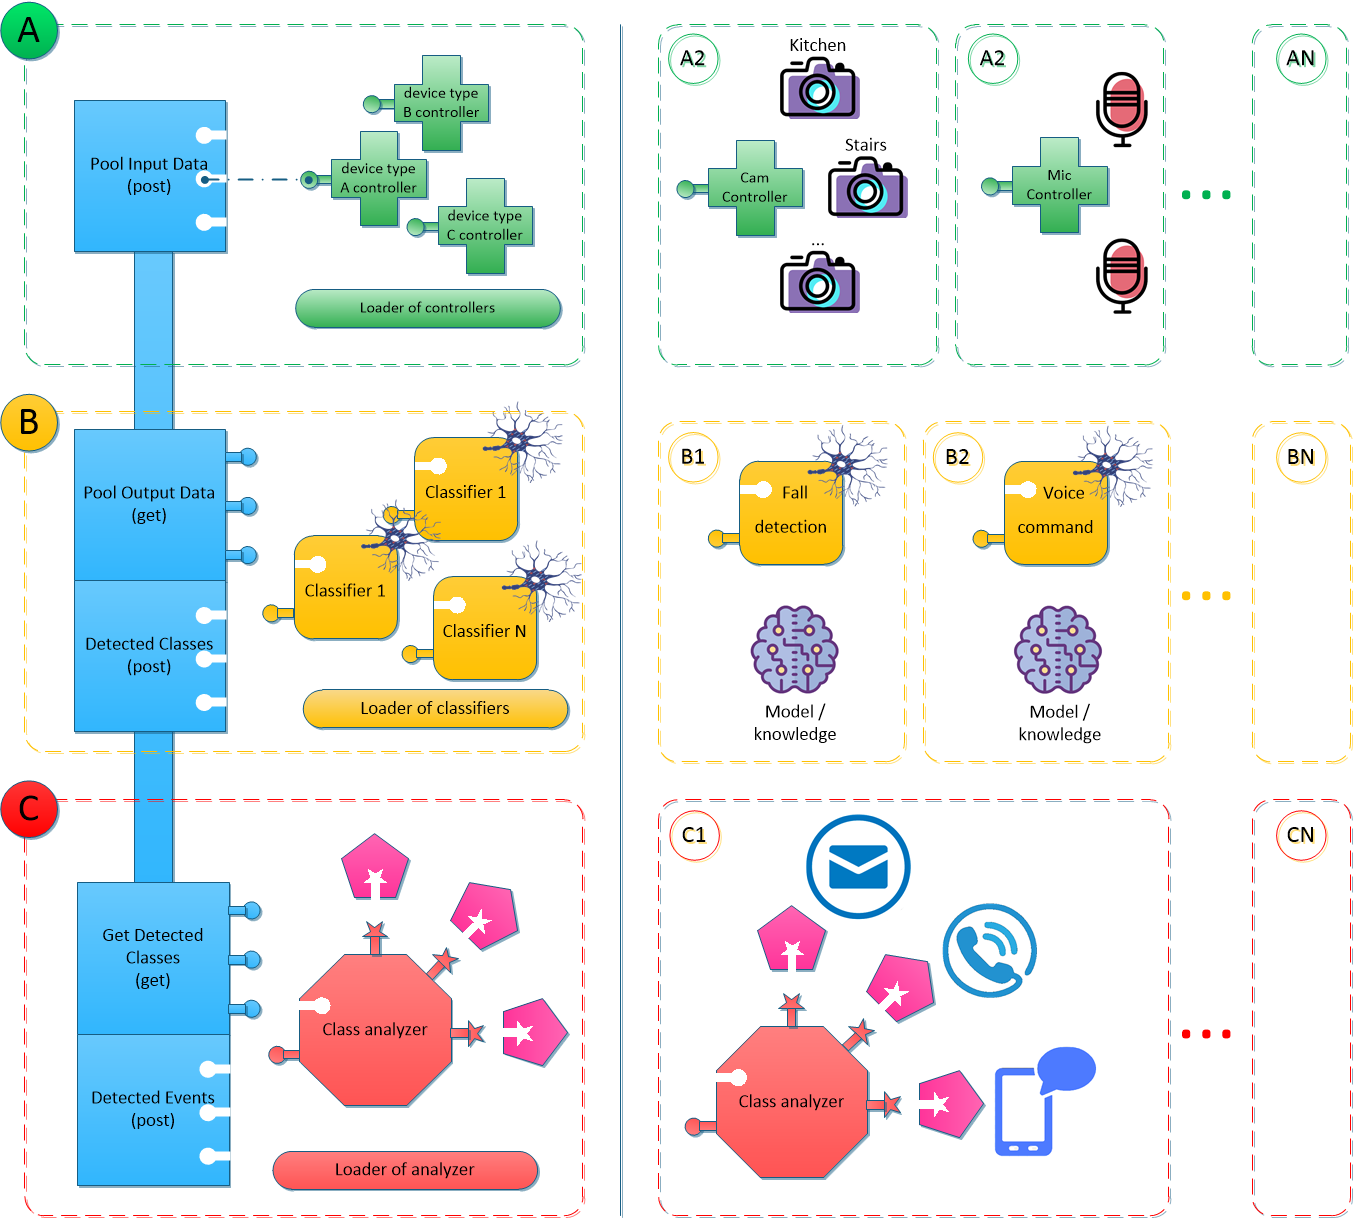
\includegraphics[width=0.8\linewidth]{imgs/03-Architecture/03-Architecture.png}
    	\caption[Diagrama general del sistema]{Diagrama general del sistema. Presenta las secciones en que se divide el sistema y los componentes que conforman cada sección. También presenta, la relación que hay entre cada componente y el sistema general para el intercambio de datos.}
	    \label{fig:Architecture}
    \end{figure}%

    \textbf{Sección A}, encargada de capturar la información de entrada (por ejemplo imágenes de una cámara web) y entregarla a la pila de datos para que otros componentes puedan hacer uso de ella. Adicionalmente, en esta sección se incluyen etapas de preparación de los datos a analizar, esto es, dar una estructura estándar a los datos sin importar el origen, de esta forma se mantendrán estructuras claramente definidas para que los componentes posteriores puedan entenderlas. El funcionamiento detallado de esta sección será explicado más adelante en la sección \ref{Sec:InputData}.

    \textbf{Sección B}, encargada de la interpretación de los datos entregados por la sección A, es aquí donde se realiza una primera identificación de eventos. La sección B consulta en la pila los datos entregados por la sección A y los procesa de forma paralela, en búsqueda de eventos concretos. Al finalizar el proceso, los eventos detectados son entregados, a la pila de datos, como una lista de pequeñas frases con la información referente al tipo de evento, el momento y la fuente. El funcionamiento detallado de esta sección será explicado más adelante en la sección \ref{Sec:HAR}.

    \textbf{Sección C}, encargada del discernimiento de las frases generadas de la sección B, identificando los eventos que deberán emitir alertas. A diferencia de los componentes de la sección B, que solo realizarán su procesamiento usando el entrenamiento previo, la sección C cuenta con un componente llamado “Analizador de eventos” el cual continúa su aprendizaje durante todo el funcionamiento del sistema. Dentro de esta sección se encuentran tanto los componentes de análisis de eventos como los notificadores, el funcionamiento detallado de esta sección será explicado más adelante \ref{Sec:Analyzer}.

    \textbf{La pila de datos} es la columna vertebral del sistema. Se encargada de controlar toda la información que fluye en el sistema y ser el medio de comunicación, permitiendo a los demás componentes enviar y consultar la información, mediante la exposición de un API\index{API}. Por tanto, la pila de datos es el único componente transversal a todo el sistema, como se muestra en la figura \ref{fig:Architecture}. El funcionamiento detallado de este componente será explicado más adelante en la sección \ref{Sec:DataPool}. 
    
    \newpage
  
\section{Pila de datos}
\label{Sec:DataPool}
    Para lograr un procesamiento altamente distribuido y un software altamente desacoplado, es necesario que el sistema tenga una forma rígida para transmitir y compartir su información. La pila de datos es la columna vertebral del sistema, es a través de ésta que fluye toda la información del sistema.
    
    La pila de datos consiste en una base de objetos de tipo \textit{Data} (explicada más posteriormente en la sección Estructura de datos \ref{sub:DataEstructure}), donde se almacenará toda la información que fluye a lo largo del sistema. Así mismo, es la implementación del patrón de instancia única (ver \ref{sub:FrameSingleton}), por lo que solo existirá una única pila de datos accesible por todos los módulos del sistema.
        
    Las tareas de la pila de datos como pieza estructural del sistema van más allá que solo tener los datos. Este componente se encarga de almacenar y administrar el acceso a los datos que serán usados por los demás componentes. Para ello se apoya en la implementación de un servicio REST\index{REST} basado en el paquete de python: "flask" (ver \ref{sub:FrameFlask}) para proveer cuatro rutas: ``\textbf{/api/tickets}'', ``\textbf{/api/events}'', ``\textbf{/api/alerts}'' y ``\textbf{/api/logs}''. 
    
    \begin{itemize}
        \item \textbf{/api/tickets}: se encarga de recibir y transmitir la información entregada por los componentes de entrada de datos (Controllers, \ref{Sec:InputData}).
        \item \textbf{/api/events}: se encarga de recibir y transmitir la información generada por los componentes de reconocimiento de actividades (Classifier, \ref{Sec:HAR}).
        \item \textbf{/api/alerts}: se encarga de recibir y transmitir la información generada por los componentes analizadores de la actividades (Analyzers, \ref{Sec:Analyzer}).
        \item \textbf{/api/logs}: se encarga de recibir información sobre sucesos o errores dentro de los diferentes componentes del sistema, de forma que se pueda tener una bitácora de la salud de todo el sistema.
    \end{itemize}
    
    En relación con lo anterior, la pila de datos cuenta con tres clases principales, 
    \textbf{Data}\index{Data structure},
    \textbf{DataPool}\index{DataPool} y 
    \textbf{CommPool}\index{CommPool}. 
    
    \begin{itemize}
        \item \textbf{Data}: está encargada de definir la estructura básica de toda la información que fluye hacia o desde la pila de datos como se detallará en la sección \ref{sub:DataEstructure}.
        \item \textbf{DataPool}: se encarga de recibir, mantener, entregar y remover la información disponible en el sistema, como se presenta en sección \ref{sub:Pool}.
        \item \textbf{CommPool}: es una clase reutilizable por los módulos que interactúan con el la pila de datos. Contiene la lógica necesaria para la comunicación entre módulos y pila de datos.
    \end{itemize}
    
    \subsection{Estructura de datos}
    \label{sub:DataEstructure}
    
        La definición de una estructura, aunque estática en los atributos que la componen, pero flexible en cuanto a la forma de la información de algunos atributos, permite la estabilidad y la escalabilidad. Por esto, la importancia subyacente de la clase \textbf{\textit{Data}} donde se define la estructura de la entidad mínima de información de todo el sistema. La tabla \ref{Tab:DataEstructureAttr} muestra los atributos que componen la clase \textbf{\textit{Data}}.
        
        \begin{table}[ht!]
        \caption[Atributos de datos a transmitir]{Atributos de la estructura de los datos que viajan por el sistema.}
        \label{Tab:DataEstructureAttr}
        \centering
        \begin{tabular}{ | l p{11cm} | } 
            \hline
             \textbf{Atributo}      & \textbf{Descripción} \\ 
            \hline\hline
            \textbf{id*}            & Identificador único del dato. Puede ser alterado al cargar a la pila (ver sección \ref{sub:Pool}). \\
            \hline
            \textbf{born*}          & Almacena la hora en que el objeto fue creado y, con esto poder controlar el tiempo de vida del dato (ver sección \ref{sub2:PoolKeepDropData}). \\
            \hline
            \textbf{source\_type}   & Identifica el tipo de dato almacenado, este puede ser CONTROLLER, CLASSIFIER, ANALYZER. \\
            \hline
            \textbf{source\_name}    & Nombre del componente o módulo que genera el dato, por ejemplo:  camController, infarctRecognizer, ventAnalyzer (ver secciones \ref{sub:DeviceController}, \ref{sub:ClassifierHAR}, \ref{sub:EventAnalyzer}). \\
            \hline
            \textbf{source\_item}   & Fuente primordial de la información, ejemplo: LivingRoom-Cam1. \\
            \hline
            \textbf{package}        & Cuando se recibe un dato desde un dispositivo, este puede ser preprocesado antes de ser enviado a la pila de datos, por ejemplo una imagen puede ser convertida a grises, con lo cual se puede tener más de una versión del mismo dato. El atributo ``package'' almacena un identificador que permite agrupar varios datos provenientes de un mismo origen. \\
            \hline
            \textbf{data}           & Este atributo contiene la información como tal, por ejemplo, si es una imagen contendrá la matriz de píxeles. No está restringido a una estructura rígida sino que cada componente de entrada podrá organizar los datos a conveniencia. \\
            \hline
            \textbf{aux}            & Permite almacenar información adicional, como la forma en que se organizan los datos o cualquier otro dato a conveniencia. \\
            \hline
            \textbf{state*}         & El estado permite controlar la vigencia del dato: ACTIVE o QUARANTINE. \\
            \hline
        \end{tabular}
        
        {(*) Indica que el valor de este atributo es autogenerado al momento de crear el dato.}
        \end{table}
        
        Además de los atributos como tal, la clase \textbf{\textit{Data}} cuenta con un método que permite serializar los datos (ver alg. \ref{Alg:getJson}), para ser transmitidos de forma plana sin importar la estructura interna. Utilizando la notación JSon\index{JSon} como formateador los datos son transmitidos y almacenados (ver alg. \ref{Alg:DataStructure}). Así pues, cualquier dato puede ser serializado para transmitir invocando el método \textbf{\textit{getJson()}}. Y en sentido inverso se puede crear el objeto a partir de una cadena de texto que contenga un JSon\index{JSon} que permita representar la clase \textbf{\textit{Data}}, invocando el método \textbf{\textit{parse(str)}} (ver alg. \ref{Alg:parse})
        
        \begin{lstlisting}[language=Python, caption={Firma del método ``\textit{getJson}'' de la clase Data.}, label=Alg:getJson, numbers=none]
def getJson(self):
            \end{lstlisting}
            
        \begin{lstlisting}[language=Python, caption={Firma del método ``\textit{parse}'' de la clase Data.}, label=Alg:parse, numbers=none]
def parse(self, str):
            \end{lstlisting}
        
        \lstinputlisting[language=Python, caption={Estructura de datos en JSon.}, label=Alg:DataStructure]{code/03-Architecture/03-DataStructure.py}
        
    Adicionalmente, la clase \textbf{\textit{Data}} provee tres métodos utilitarios: Alroritmos \ref{Alg:signatureValueOf}, \ref{Alg:signatureSerialize} y \ref{Alg:signatureDeserialize}.
    
    \begin{itemize}
                \item \textbf{\textit{valueOf}} (alg. \ref{Alg:signatureValueOf}): Permite obtener el valor de un atributo a partir de su nombre.
                \begin{lstlisting}[language=Python, caption={Firma del método "\textit{valueOf}" de la clase Data.}, label=Alg:signatureValueOf, numbers=none]
def valueOf(self, key):
                \end{lstlisting}

                \item \textbf{\textit{serialize}} (alg. \ref{Alg:signatureSerialize}): Permite que cualquier componente pueda, de forma simplificada, serializar los datos, sin importar su forma, para poder enviarlos al servicio de la pila de datos en forma de cadena de texto.
                \begin{lstlisting}[language=Python, caption={Firma del método "\textit{serialize}" de la clase Data.}, label=Alg:signatureSerialize, numbers=none]
def serialize(self, data:Any):
                \end{lstlisting}
                
                \item \textbf{\textit{deserialize}} (alg. \ref{Alg:signatureDeserialize}): Permite que cualquier componente pueda, de forma simplificada, convertir un cadena de texto recibida desde la pila de datos a su estructura original.
                \begin{lstlisting}[language=Python, caption={Firma del método "\textit{deserialize}" de la clase Data.}, label=Alg:signatureDeserialize, numbers=none]
def deserialize(self, data:str):
                \end{lstlisting}
    \end{itemize}
    
    \subsection{Transmisión y vigencia de datos}
    \label{sub:Pool}
        Una vez iniciado el servicio de la pila de datos (\textbf{\textit{DataPool}}) se exponen los métodos (verbos) \textit{post} y \textit{get}, en las rutas ``\textbf{/api/tickets}'', ``\textbf{/api/events}'', ``\textbf{/api/alerts}'' y ``\textbf{/api/logs}'', para el flujo de información de todo el sistema, como se ve en la figura \ref{fig:ModuleComunication}. Cada una de las rutas es gestionada por una clase independiente y homónima a la ruta que gestiona.
        
        \begin{figure}[ht!]
        	\centering
        	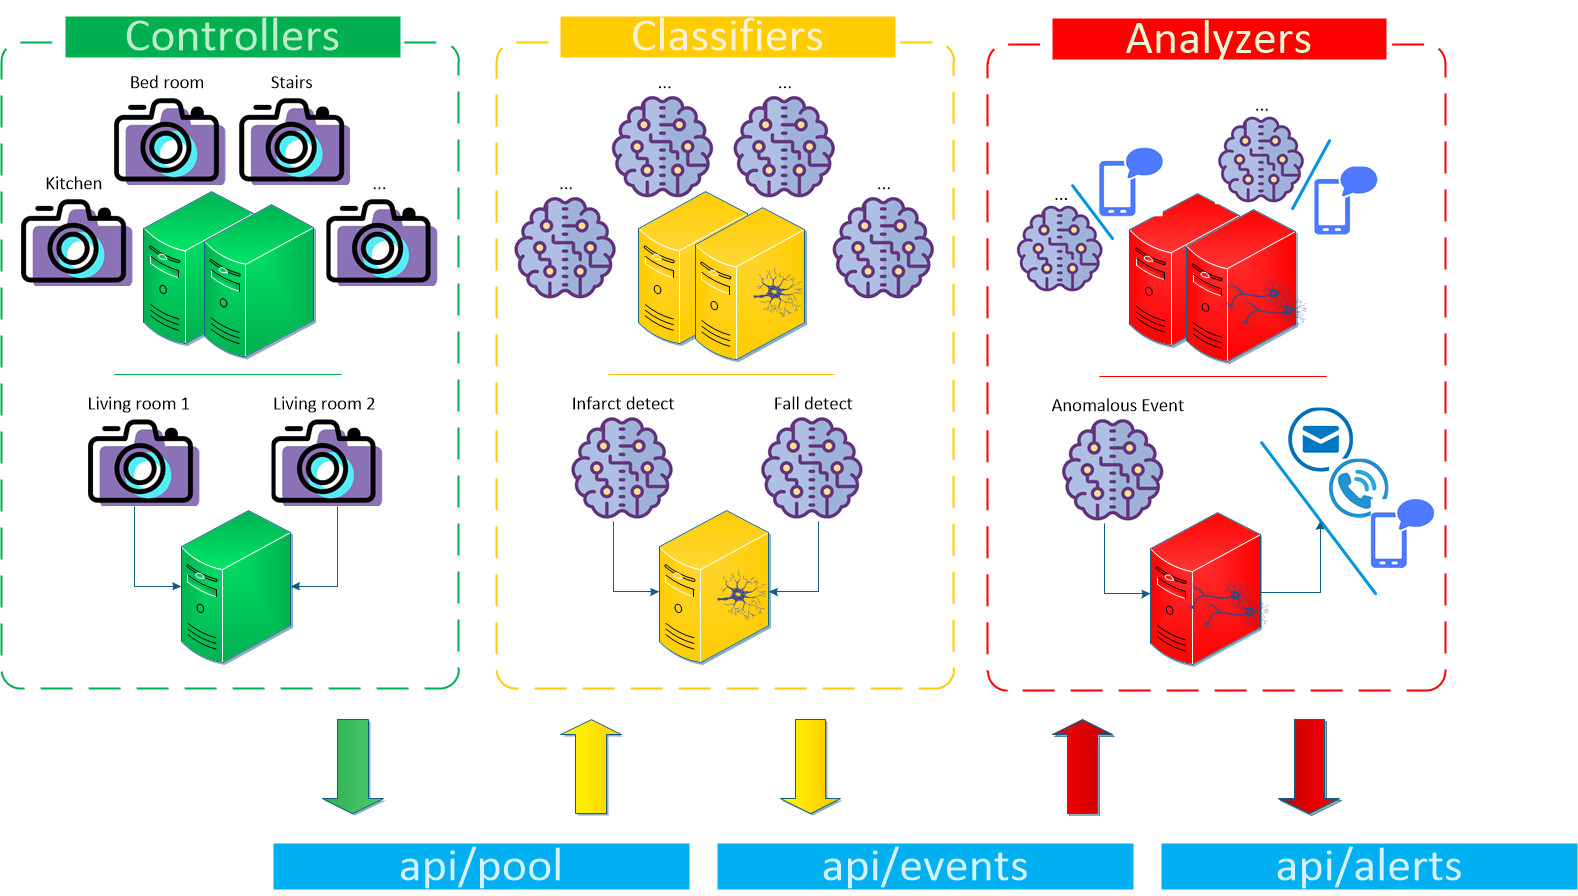
\includegraphics[width=0.8\linewidth]{imgs/03-Architecture/03-Communication.png}
        	\caption[Flujo general de información del sistema]{Flujo general de información del sistema. De izquierda a derecha se presenta como fluye la información desde su captura hasta la detección de eventos, pasando por las tres rutas definidas para el sistema.}
    	    \label{fig:ModuleComunication}
        \end{figure}%
        
        Para unificar y facilitar la comunicación entre los módulos y la pila de datos, en este trabajo se desarrollo la clase \textbf{\textit{CommData}}. Esta clase expone los métodos que se detallaran a continuación, para, además, agilizar el desarrollo de nuevos componentes:
        \begin{itemize}
                \item \textbf{\textit{send}} (alg. \ref{Alg:sendData}): Permite enviar de forma simple un objeto data a la pila de datos. Siendo \textit{data} el objeto a almacenar en la pila de datos. Es importante mencionar que el objeto recibido podría tener valor solamente en su atributo data, ya que los demás atributos, en caso de ir vacíos serán cargados automáticamente con los valores del archivo de configuración del componente. 
                \begin{lstlisting}[language=Python, caption={Firma del método "\textit{sendData}" de la clase \textbf{\textit{CommPool}}.}, label=Alg:sendData, numbers=none]
def send(self, data:Data):
                \end{lstlisting}
                \item \textbf{\textit{receive}} (alg. \ref{Alg:sendData}): Permite enviar de forma simple un objeto data a la pila de datos. Siendo \textit{data} el objeto con los criterios de filtrado, \textit{limit} la cantidad de datos a retornar (-1 para no considerar este filtro) y \textit{lastTime} una variable de tiempo que indica la ultima vez que se consulto la pila de datos (-1 para no considerar este filtro).
                \begin{lstlisting}[language=Python, caption={Firma del método "\textit{receive}" de la clase \textbf{\textit{CommPool}}.}, label=Alg:receiveData, numbers=none]
def receive(self, data:Data, limit=-1, lastTime=-1):
                \end{lstlisting}
                
                \item \textbf{\textit{log}} (alg. \ref{Alg:signatureLog}): 
                Permite que cualquier componente pueda, de forma simplificada, enviar mensajes a la bitácora del sistema, pudiendo ser estos Errores, Advertencias, Información o cualquiera de la lista de opciones disponible en por el numerador ``\textit{LogTypes}''. Siendo \textit{data} un objeto con la misma estructura utilizan los componentes para la comunicación con la pila de datos, que en su atributo data contiene el mensaje a almacenar.
                \begin{lstlisting}[language=Python, caption={Firma del método "\textit{log}".}, label=Alg:signatureLog, numbers=none]
def log(self, data:Data, type:):
                \end{lstlisting}
        \end{itemize}
        
        Independientemente de la clase \textbf{\textit{CommPool}}, la pila de datos como tal expone los servicios de comunicación con los diferentes componentes dos sentidos:  \textbf{Recibir datos} y \textbf{Entregar datos}. El primer caso ocurre cuando los módulos envían información a la pila de datos y el segundo caso es cuando la consultan.

        \subsubsection{Recibir datos}
        \label{sub2:PoolPost}
            Para que la pila de datos reciba la información se usa el método \textit{post} de cada una de las rutas. Este método recibirá como parámetro un objeto que cumpla con la estructura de la clase \textbf{\textit{Data}}\index{Data Estructure}. En el algorigmo \ref{Alg:PoolPostParams} se presenta un ejemplo de la estructura que tendría la petición.
            
            \lstinputlisting[language=Python, caption={Ejemplo de parámetros para enviar datos la pila.}, label=Alg:PoolPostParams]{code/03-Architecture/03-PoolPostParams.py}
            
            Cada vez que el método \textit{post} es invocado, se crea un objeto con la estructura \textbf{\textit{Data}} (ver sección \ref{sub:DataEstructure}). 
            
            Como se mencionó anteriormente, al momento de crear el objeto \textbf{\textit{Data}} se asigna un identificador único dentro del sistema, además se adiciona la hora en que se creo y el estado. Adicionalmente, dependiendo la ruta utilizada, el atributo source\_type será cambiado por el tipo asociado a cada una así: 
            
            \begin{itemize}
                \item api/tickets => CONTROLLER
                \item api/events  => RECOGNIZER
                \item api/alerts  => ANALYZER
            \end{itemize}
        
        \subsubsection{Entregar datos}
        \label{sub2:PoolGet}
            Todo dato recibido, siempre que éste no haya cumplido su tiempo de vida, estará disponible para ser consultado por cualquier componente. Para ello se expone el método \textit{get} en cada ruta. 
            
            Para poder consultar información alojados en la pila de datos, es necesario entregar parámetros al método get. En este caso los parámetros serán usados como filtro de la información, por ejemplo si un componente de reconocimiento de eventos simples (ver sección \ref{Sec:HAR}), desea procesar solo los datos de un dispositivo específico debe indicarlo dentro de los parámetros enviados. La tabla \ref{Tab:PoolGetParams} presenta los parámetros recibidos por el método y en el fragmento de código \ref{Alg:PoolGetParams} se muestra un ejemplo.
            
            \begin{table}[ht!]
            \caption[Parámetros para consultar datos de la pila]{Parámetros para consultar datos de la pila.}
            \label{Tab:PoolGetParams}
            \centering
            \begin{tabular}{ | l p{11cm} | } 
                \hline
                 \textbf{Atributo}      & \textbf{Descripción} \\ 
                \hline\hline
                \textbf{id}             & identificador único del dato. \\
                \hline
                \textbf{package}        & Retorna todos los datos que tienen un mismo origen. \\
                \hline
                \textbf{source\_type}   & Identifica el tipo de dato almacenado, este puede ser: CONTROLLER para la subruta \textbf{api/tickets}, RECOGNIZER para la subruta \textbf{api/events} y ANALYZER para la subruta \textbf{api/alerts}.\\
                \hline
                \textbf{source\_name}    & Nombre del componente o módulo que genera el dato. Puede ser una expresión regular, por ejemplo 'camController' para un módulo específico o 'CamController*?' para los datos de cualquier controlador que inicie con 'CamController'. \\
                \hline
                \textbf{source\_item}   & Fuente primordial de la información. Puede ser una expresión regular, por ejemplo 'LivingRoom-Cam1' para un dispositivo específico o 'Living*?' para los datos de cualquier dispositivo que cuyo nombre inicie con 'Living'. \\
                \hline
                \textbf{limit}          & Limita la cantidad de elementos a retornar \\
                \hline
                \textbf{lastTime}        & Es el tiempo de la ultima consulta, si se envía solo retornará datos creados posterior a ese momento \\
                \hline
            \end{tabular}
            \\{(*) Todos los atributos son opcionales.}
            \end{table}
            
            \lstinputlisting[language=Python, caption={Ejemplo de parámetros para consultar la pila.}, label=Alg:PoolGetParams]{code/03-Architecture/03-PoolGetParams.py}
            
            Dado que todos los parámetros son opcionales, el método puede ser invocado incluso sin parámetros, en tal caso no se aplicará ningún filtro y se retornarán todos los datos vigentes, es decir, que no se hayan etiquetados para eliminar (ver sección \ref{sub2:PoolKeepDropData}).
            
            Para reducir la redundancia de procesamiento y permitir que cada componente funcione de forma asíncrona con los demás, este método además de entregar los datos vigentes y que cumplen con los criterios de filtrado, entrega una variable llamada "\textit{timeQuery}" que contiene el momento (hora en la máquina donde se ejecuta el servicio) en que fue consultado. De esta forma siempre se puede solicitar solo los datos más recientes que la última consulta hecha. Así pues, los datos retornados son una lista de objetos con la estructura definida en la sección \ref{sub:DataEstructure}, más el "\textit{timeQuery}".

        \subsubsection{Permanencia y eliminación de datos}
        \label{sub2:PoolKeepDropData}
        
            La clase \textbf{\textit{DataPool}} se encarga de la permanencia y gestión de los datos. Esta clase mantiene la base de datos con toda la información recibida por el sistema.
            
            La pila de datos tiene una política de permanencia de datos basado en tiempos (ver fig. \ref{fig:PoolFlow}). Que mantiene el sistema en estado óptimo de forma constante.
            
            \begin{figure}[ht!]
            	\centering
            	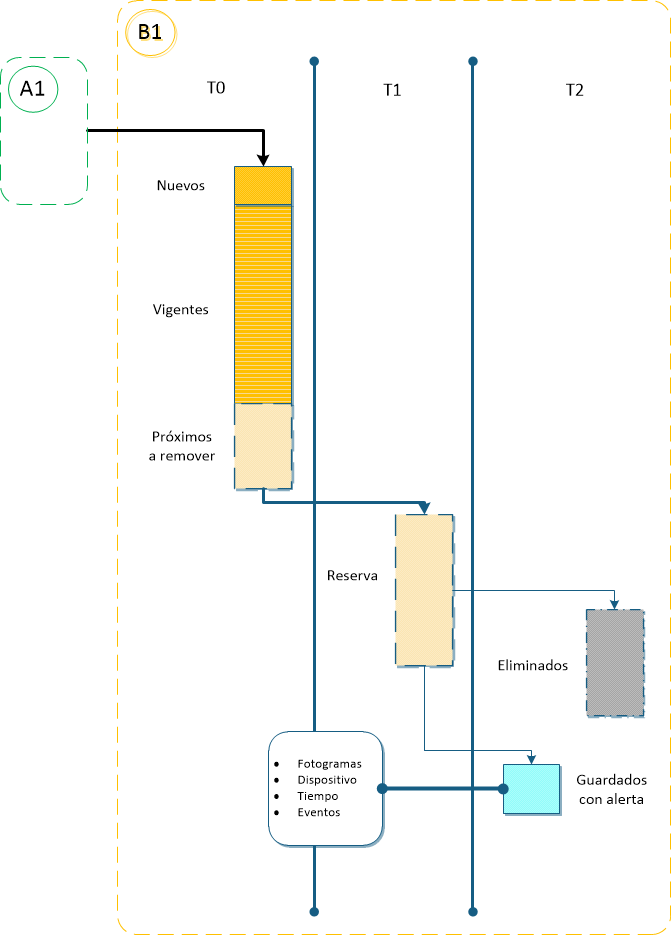
\includegraphics[width=0.8\linewidth]{imgs/03-Architecture/03-DataPool.png}
            	\caption[Diagrama de la pila de datos]{Diagrama de la pila de datos. Presenta los diferentes estadios por los que pasa un dato desde su creación hasta su eliminación del sistema.}
        	    \label{fig:PoolFlow}
            \end{figure}%
        
            Como se muestra en la figura \ref{fig:PoolFlow}, los datos recibidos se apilan y la enmarcan en ventanas de tiempo, para que los módulos los puedan consultar. La primera ventana de tiempo mantendrá los datos apilados por orden de llegada y los irá entregando por demanda, considerando la última vez que un componente consultó la pila. 
            
            Una vez cumplida la ventana de tiempo los datos serán removidos de la pila de datos vigentes, pero se mantendrán durante un periodo adicional en reserva, en caso de que una alerta sea reportada por el analizador de eventos, si es así se almacenará de forma permanente con la información complementaria de tiempo, dispositivo y eventos detectados. En caso de no generar ninguna alerta, los datos recibidos serán eliminados definitivamente.

        \subsubsection{Métodos adicionales de la pila de datos}
        \label{sub2:PoolAditional}
            Dentro de cada una de las subrutas se adicionó un tercer verbo (\textbf{\textit{put}}), que permite invocar algunos métodos adicionales de la pila de datos (ver patrón comando en \ref{sub:FrameCommand}). Para invocar este método es suficiente con enviar como parámetro la variable ``\textit{command}'' con el nombre de la acción a ejecutar. La tabla \ref{Tab:PoolPutParams} muestra los posibles valores que puede tomar ``\textit{command}''.
            
            \begin{table}[ht!]
            \caption[Métodos adicionales del la pila]{Métodos adicionales del la pila.}
            \label{Tab:PoolPutParams}
            \centering
            \begin{tabular}{ | l p{11cm} | } 
                \hline
                 \textbf{Valor}               & \textbf{Descripción} \\ 
                \hline\hline
                \textbf{time}     & Retorna la hora actual del servidor. \\
                \hline
                \textbf{isLive} & Permite una rápida verificación del estado del la pila. \\
                \hline
                \textbf{pop}     & Permite invocar la purga de los datos de la pila, eliminando los datos que ya no cumplen con la ventana de tiempo de vigencia (ver sección \ref{sub2:PoolKeepDropData}). \\
                \hline
                \textbf{count}       & Entrega el número total de datos almacenados en la pila. \\
                \hline
            \end{tabular}
            \\{(*) Cualquier valor diferente dará como resultado un mensaje indicando el error.}
            \end{table}
            
            Además de los presentados, la clase \textbf{\textit{CommPool}}, tiene algunos métodos utilitarios que pueden ser invocados sin tener llamar el servicio directamente \index{REST}. Estos métodos son:
            
            \begin{itemize}
                \item \textbf{\textit{sendCommand}} (alg. \ref{Alg:signatureSendCommand}): Permite que cualquier componente pueda invocar de forma simplificada alguno de los métodos adicionales de la pila de datos (ver tab. \ref{Tab:PoolPutParams}).
                \begin{lstlisting}[language=Python, caption={Firma del método "\textit{sendCommand}".}, label=Alg:signatureSendCommand, numbers=none]
def sendCommand(self, command):
                \end{lstlisting}

                \item \textbf{\textit{getTime}} (alg. \ref{Alg:signatureGetTime}): Permite que cualquier componente pueda, de forma simplificada, consultar la hora actual de servidor.
                \begin{lstlisting}[language=Python, caption={Firma del método "\textit{getTime}".}, label=Alg:signatureGetTime, numbers=none]
def getTime(self):
                \end{lstlisting}

                \item \textbf{\textit{getTimeDiff}} (alg. \ref{Alg:signatureGetTimeDiff}): Permite que cualquier componente pueda, de forma simplificada, consultar la diferencia (en milisegundos) entre el servidor y la máquina en que se esta ejecutando el componente.
                \begin{lstlisting}[language=Python, caption={Firma del método "\textit{getTimeDiff}".}, label=Alg:signatureGetTimeDiff, numbers=none]
def getTimeDiff(self):
                \end{lstlisting}

                \item \textbf{\textit{isLive}} (alg. \ref{Alg:signatureIsLive}): Permite que cualquier componente pueda, de forma simplificada, saber la disponibilidad del servicio de la pila de datos.
                \begin{lstlisting}[language=Python, caption={Firma del método "\textit{isLive}".}, label=Alg:signatureIsLive, numbers=none]
def isLive(self):
                \end{lstlisting}

                \item \textbf{\textit{count}} (alg. \ref{Alg:signatureCount}): Permite que cualquier componente pueda, de forma simplificada, consultar el numero de elementos almacenados en la pila de datos.
                \begin{lstlisting}[language=Python, caption={Firma del método "\textit{count}".}, label=Alg:signatureCount, numbers=none]
def count(self):
                \end{lstlisting}
            
            \end{itemize}
    
    \newpage

\section{Estructura básica de componentes extensibles}
\label{Sec:ComponentStructure}
    Como se mencionó anteriormente, en las secciones A, B y C (ver figura \ref{fig:Architecture}) se ubican los componentes que por su naturaleza pueden ser extendidos en su funcionalidad, permitiendo, incluso, la ejecución de múltiples instancias simultáneamente.
    
    Aun cuando cada uno de los componentes extensibles: Controlador de dispositivos, Clasificador de reconocimiento de actividad humana, Analizador de eventos o canales de notificación, tienen funciones claramente diferenciadas, todos fueron definidos bajo una misma estructura.
    
    \begin{figure}[ht!]
    	\centering
    	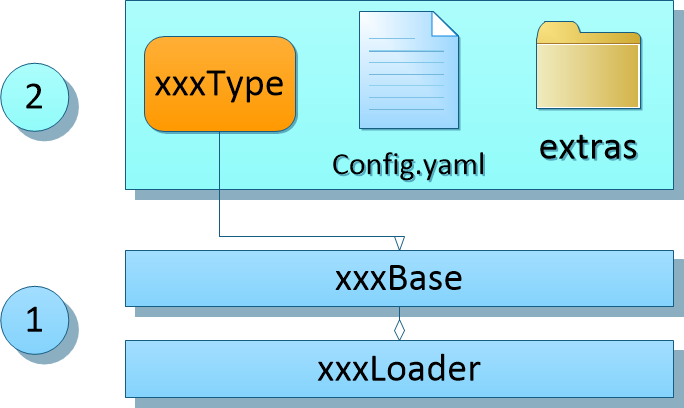
\includegraphics[width=0.8\linewidth]{imgs/03-Architecture/03-ComponentStructure.png}
    	\caption[Estructura general de un componente extensible]{Estructura general de un componente extensible. 1) Piezas de código incluidas en el núcleo del sistema. 2) Piezas de software, configuración y adicionales exclusivas de cada componente}
	    \label{fig:ComponentStructure}
    \end{figure}%
    
    La figura \ref{fig:ComponentStructure} presenta las partes de un componente extensible, en la parte 1 se presentan dos piezas encargadas de de la estructura y comportamiento general de cualquier componente y se encuentran en el núcleo del sistema. En primer lugar el cargador (Loader), encargado de identificar componentes disponibles en el sistema (que están en una ubicación definida, ver la sección de estructura de directorios para mayor claridad). El cargador es, en sí mismo, un servicio que constantemente está supervisando la ejecución de los componente y en caso de ser necesario reinicia la ejecución del que corresponda.
    
    La segunda pieza del componente incluida en el núcleo del sistema es la clase base. De igual forma que el cargador, existe una clase base para cada tipo componente, cuatro en total. La clase base esta construida como una clase abstracta que define la estructura de un componente y de esta forma generalizar la forma en que el cargador puede iniciar y monitorizar cada una. Además, cuenta con métodos genéricos implementados para la comunicación de componente con la Pila de datos.
    
    En la parte 2 de la figura \ref{fig:ComponentStructure}, se muestran las piezas especificas del componente, siendo obligatorios la clase tipo, que hereda y extiende la clase base, aportando funcionalidad específica al componente. También se encuentra en esta parte el archivo 'config.yaml' que define las variables necesarias para el correcto funcionamiento de cada componente, como pueden ser tamaños de capturas o cualquier otro necesario. Finalmente, una o varias carpetas no obligatorias, como  puede ser 'model' para guardar archivos de entrenamientos previos o cualquier otro recurso que sea necesario para el componente.
    
    Todas las clases tipo heredan de la clase ``\textbf{Component}'' que además provee funcionalidades de uso común, como son:
    
    \begin{itemize}
    
            \item \textbf{\textit{checkConnection}} (alg. \ref{Alg:checkConnection}):
            Verifica la conexión del componente con la pila de datos.
            \begin{lstlisting}[language=Python, caption={Firma del método ``\textit{checkConnection}''.}, label=Alg:checkConnection, numbers=none]
def checkConnection(self):
            \end{lstlisting}
        
            \item \textbf{\textit{log}} (alg. \ref{Alg:logComponent}):
            Permite el reporte de mensajes al registro de atediaría. Este método recibe un objeto tipo \textbf{Data}, con lo cual se obtiene toda la información del componente generador del mensaje. El método también recibe el tipo de mensaje que puede ser de Error, Alerta o Información. Este método además de presentarlo en la forma tradicional de Python, también enviará el mensaje a la Pila de datos de forma que se pueda tener una bitácora centralizada, lo cual se hace útil cuando la ejecución de los diferentes componentes del sistema se hace de forma distribuida.
            \begin{lstlisting}[language=Python, caption={Firma del método ``\textit{log}''.}, label=Alg:logComponent, numbers=none]
def log(self, data, type):
            \end{lstlisting}
        
        \end{itemize}
        
    Además de los mencionados, cada componente contendrá métodos abstractos que deberán ser implementados por cada uno y que serán comentados más adelante. Pues, aunque todos los componentes tienen la misma estructura, existen particularidades no solo el tipo del componente sino que aun componentes del mismo tipo podrían tener sus necesidades particulares.
    
    \newpage
    
\section{Sección A - Entrada de datos}
\label{Sec:InputData}
    En esta sección se encuentran las piezas principales de la captura de información. Como se muestra en el diagrama general (fig. \ref{fig:Architecture}), la información a analizar se recibe por un medio físico. Para el desarrollo de este trabajo sólo se consideraron cámaras RGB, sin embargo, el diseño del sistema permite cualquier otra fuente. 
    
        \begin{figure}[ht!]
        	\centering
        	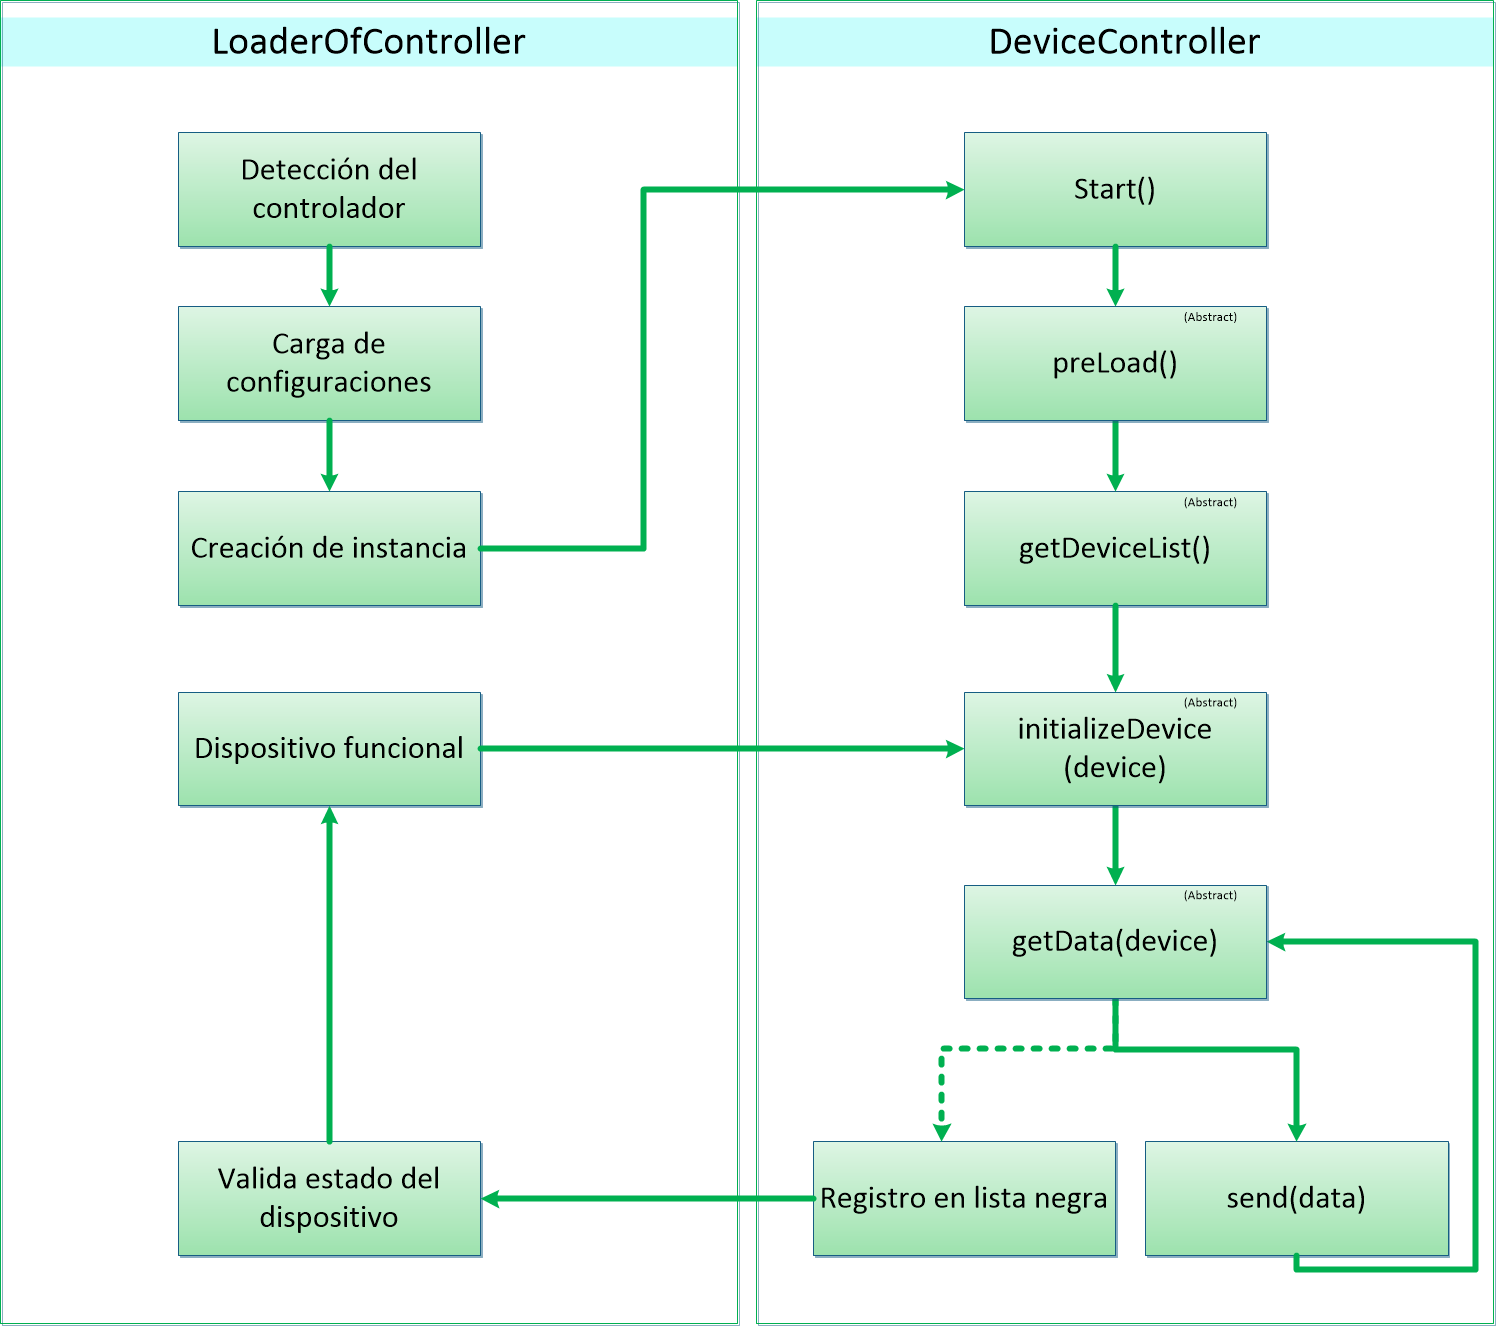
\includegraphics[width=0.9\linewidth]{imgs/03-Architecture/03-InputDataLifeCicle.png}
        	\caption[Ciclo de vida de la entrada de datos]{Ciclo de vida de la entrada de datos. A la izquierda las tareas realizadas por el cargador de controladores (LoaderOfController). A la derecha las tareas realizadas por el controlador del dispositivo (DeviceController).}
    	    \label{fig:InputDataLifeCicle}
        \end{figure}%
    
    Esta sección de sistema consta de dos artefactos principales: El cargador de controladores y los controladores de dispositivo (ver figura \ref{fig:InputDataLifeCicle}). Mediante la combinación de ambos se captura y organiza la información para que se entregue de forma homogénea a la pila de datos. 
    
    \subsection{ cargador de controladores - LoaderOfController}
    \label{LoaderController}
        Esta clase se basa en definición del patrón ``método factoría'' y cumple tres funciones principales, primero identifica que controladores de dispositivos están disponibles, luego carga e inicia la captura de datos y por último se asegura que los controladores se mantengan en funcionamiento.
        
        \subsubsection{Detección de controladores de dispositivos}
        \label{sub2:InputDeviceDetection}
            Cuando el cargador de controladores es inicializado recorre la carpeta ``Controllers'' en búsqueda de archivos con nombre ``config.yaml''. De esta forma, toda sub carpeta dentro de ``Controllers'' que contenga un archivo de configuración, será considerado un posible componente a cargar.
            
            Como se mostró en la se sección \ref{Sec:ComponentStructure} cada componente de entrada debe contar con un archivo ``config.yaml'', el cual permitirá al cargador de controladores identificar características como la clase que debe ser inicializada para cargar el componente además de parámetros particulares.
            
            Para tomarlo como un componente válido, el archivo de configuración debe cumplir con los criterios expuestos en la sección \ref{Sec:ComponentStructure}, asegurando además que el estado del mismo esté asignado como ``Activo'' (Enabled). 
            
            Adicionalmente, el archivo ``config.yaml'' contará con dos variables adicionales: 'CHECKING\_TIME' y 'SAMPLING'. La primera permite definir el tiempo de espera para verificar el funcionamiento un dispositivo, en caso de que se haya detectado un fallo. La segunda, permite definir la tasa de muestreo de un dispositivo, por ejemplo 30 cuadros por segundo. 
        
        \subsubsection{Inicio de controladores}
        \label{sub2:InputDeviceStarting}
            
            Gracias al uso del patrón de ``método plantilla'' (ver \ref{sub:FrameTemplateMethod}), el cargador de controladores es capaz de cargar de forma dinámica componentes que hayan sido creados en el momento que se desarrolla este sistema o posteriormente, incluso componentes que se pongan en la carpeta de ``Controllers'' después de haber iniciado el sistema, siempre que cumpla con las consideraciones que se presentan en la sección de detección de dispositivos.
            
            Una vez cargado el controlador, creado una instancia del mismo, se invoca el método \textit{start} implementado en la clase padre del componente (ver \ref{sub:DeviceController}). En adelante, el componente será gestionado por la clase ``DeviceController'', salvo que se presenté algún error no controlado y éste se detenga, en cuyo caso el cargador de controladores intentará iniciarlo nuevamente.
        
        \subsubsection{Manteniendo dispositivos funcionando}
        \label{sub2:InputDeviceKeepAlive}
            La naturaleza del sistema impone que todos sus componentes mantengan un funcionamiento constante incluso con la posibilidad de fallos. Si un dispositivo físico, por ejemplo, una cámara, presenta algún error el cargador de controladores intentará volver a iniciar el dispositivo, sin afectar el funcionamiento de los otros componentes que se ejecutan en el sistema ya que cada controlador de dispositivos se mantiene aislado de los demás.
            
            Para ello, cuando un controlador falla al obtener información de un dispositivo, lo registra en una lista negra. El cargador de controladores, cada 30 segundos recorre el listado de controladores activos (ver patrón iterador \ref{sub:FrameIterator}) revisando que dispositivos están en lista negra e intentando volver a recibir datos de ellos. En caso de tener éxito el propio Cargador de controladores retira al dispositivo de la lista negra y con ello el controlador volverá a consultar y a enviar datos a la pila.
            
            Adicionalmente, este componente es capaz, en cualquier momento y de forma automática, de detectar cambios en el archivo de configuración, recargando el controlador del dispositivo con sus nuevas configuraciones. 
    
    \subsection{Controlador de dispositivos - DeviceController}
    \label{sub:DeviceController}
        El controlador de dispositivos será el encargado de comunicarse directamente con los dispositivos físicos y, por tanto, podrá existir al menos un módulo de este tipo por cada tipo de dispositivo a usar, por ejemplo: un controlador para cámaras RGB, uno para sensores kinects, etc.
        
        Es importante indicar que, debido al diseño del sistema, cada controlador de dispositivos podrá ser ejecutado en máquinas independientes, esto permite que varias instancias del componente ejecutándose al mismo tiempo, permitiendo por ejemplo, varias cámaras capturando imágenes en diferentes ordenadores y enviándolas concurrentemente a la pila de datos. Además, este trabajo cuenta una plantilla (sección \ref{Sec:DeviceControllerTemplate}), que se presentará en detalle más adelante, con la cual se podrán construir otros controladores de dispositivos, de forma que el sistema pueda escalar y pueda tener compatibilidad con nuevos dispositivos o fuentes de datos.
        
        El controlador de dispositivos se basa en la implementación de una clase abstracta (clase padre) que define las reglas para la construcción de un controlador para un dispositivo específico. De esta forma, cualquier controlador de un dispositivo debe heredar de la clase abstracta ``DeviceController'', obligándole a implementar algunos métodos específicos, aunque también se cuenta con algunos previamente implementados. Los siguientes métodos serán presentados siguiendo el ciclo de vida de la captura de datos presentada en la figura \ref{fig:InputDataLifeCicle}. 
    
        \begin{itemize}
        
            %  --- Start Controller
            \item \textbf{\textit{start}} (alg. \ref{Alg:startDevice}): 
            Inicia el controlador como tal. Inicia el registro de actividad en los log del sistema. Se encarga de invocar sucesivamente los demás métodos del ciclo de vida de la entrada de datos. 
            
            Un componente puede iniciar de dos formas: independiente o conectado, en el primer caso no se enviarán los datos la pila de datos sino que se presentarán directamente mediante el método \textbf{\textit{showData}}. En caso de iniciar conectado, el método \textbf{\textit{start}} comprueba la conectividad con la pila de datos.
            
            Finalmente, este método inicia los mecanismos para estar en constante revisión del funcionamiento del dispositivo y en caso de se fallo, pone el dispositivo en cuarentena hasta asegurar el funcionamiento del mismo, de esta forma se aíslan los fallos de un dispositivo y que no afecte a los demás. 
            
            \begin{lstlisting}[language=Python, caption={Firma del método ``\textit{start}''.}, label=Alg:startDevice, numbers=none]
def start(self):
            \end{lstlisting}
        
            %  --- PreLoad Controller
            \item \textbf{\textit{preLoad}} (alg. \ref{Alg:preLoadDevice}):
            (abstracto) Método invocado justo de iniciar la captura de datos. Tiene el objetivo de cargar los recursos para la captura y pre procesamiento de los datos.
            
            \begin{lstlisting}[language=Python, caption={Firma del método \textit{preLoad} de DeviceController.}, label=Alg:preLoadDevice, numbers=none]
@abc.abstractmethod
def preLoad(self):
            \end{lstlisting}
            
            %  --- getDeviceList Controller
            \item \textbf{\textit{getDeviceList}} (alg. \ref{Alg:getDeviceList}):
            (abstracto) Retorna el listado de dispositivos físicos disponibles, además cada dispositivo podrá tener una etiqueta para el reconocimiento, por ejemplo ``LivingRoom1'', ``Kitchen'', etc. Para ello se lee el archivo de configuración de componente (ver sección \ref{sub2:devicesFileController}). 
            \begin{lstlisting}[language=Python, caption={Firma del método ``\textit{getDeviceList}''.}, label=Alg:getDeviceList, numbers=none]
def getDeviceList(self):
            \end{lstlisting}
            
            %  --- inicialiceDevice Controller
            \item \textbf{\textit{initializeDevice}} (alg. \ref{Alg:initializeDevice}):
            (abstracto) Método que activa cada dispositivo físico e inicia la captura datos. 
            
            \begin{lstlisting}[language=Python, caption={Firma del método ``\textit{initializeDevice}''.}, label=Alg:initializeDevice, numbers=none]
@abc.abstractmethod
def initializeDevice(self, device):
            \end{lstlisting}
            
            %  --- getData Controller
            \item \textbf{\textit{getData}} (alg. \ref{Alg:getDataDevice}):
            (abstracto) Este método Retorna los datos capturado del dispositivo físico (\textit{idDevice}).
            
            Este método retorna una lista de objetos de tipo \textbf{\textit{Data}}, pues es posible realizar pre procesamiento a los datos capturados, antes de enviarlos a la pila de datos, con esto es posible obtener de una captura, por ejemplo, la imagen RGB original más una en grises o incluso cambios más sofisticados como la extracción de la persona del fondo de la imagen.
            
            En caso de que a los datos capturados se aplique algún procesamiento adicional, todos contendrán un mismo valor en el atributo ``package'' de los objetos retornados. Además en el atributo ``source\_name'' tendrá el nombre del componente y separado por una barra ('/'), el nombre que identifica el proceso realizado, por ejemplo, ``CamController/Gray'' para imágenes convertidas a escala de grises. Esto se tendrá en cuenta cuando algún componente consulte datos en la pila de datos.
            
            \begin{lstlisting}[language=Python, caption={Firma del método ``\textit{getData}''.}, label=Alg:getDataDevice, numbers=none]
@abc.abstractmethod
def getData(self, device):
            \end{lstlisting}
            
            %  --- send Controller
            \item \textbf{\textit{send}} (alg. \ref{Alg:sendDevice}): 
            Serializa los datos y envía a la pila de datos.
            
            \begin{lstlisting}[language=Python, caption={Firma del método ``\textit{send}''.}, label=Alg:sendDevice, numbers=none]
def send(self, controller, device, data, aux=None, package=''):
            \end{lstlisting}
            
            %  --- check Controller
            \item \textbf{\textit{check}} (alg. \ref{Alg:checkController}): 
            (abstracto) En caso de que el dispositivo físico tenga algún problema y se detenga, se intentará comprobar con esta función, que el dispositivo vuelva estar estar disponible y, en tal caso, volver a cargar datos.
            
            Este método retornara un valor de ``Verdadero'' o ``Falso'' indicando si el dispositivo esta funcionando correctamente.
            
            \begin{lstlisting}[language=Python, caption={Firma del método ``\textit{check}''.}, label=Alg:checkController, numbers=none]
def check(self, device):
            \end{lstlisting}
        
        \end{itemize}
        
        Además de los métodos mencionados, la clase ``DeviceController'' espera la implementación de algunos métodos adicionales.
        
        \begin{itemize}
            
            %  --- showData Controller
            \item \textbf{\textit{showData}} (alg. \ref{Alg:showDataDevice}):
            (Abstracto) Este método es útil para presentar los datos capturados por el dispositivo, cuando el componente inicia de forma independiente. Este método será invocado en lugar del método \textbf{\textit{send}}.
            
            \begin{lstlisting}[language=Python, caption={Firma del método ``\textit{showData}''.}, label=Alg:showDataDevice, numbers=none]
@abc.abstractmethod
def showData(self, data):
            \end{lstlisting}
            
            %  --- Simulate Controller
            \item \textbf{\textit{simulateData}} (alg. \ref{Alg:simulateDataDevice}):
            (Abstracto) Este método es útil para simular la captura de los datos capturados por el dispositivo, cuando el componente inicia de forma independiente. Este método será invocado en lugar del método \textbf{\textit{getData}}.
            
            \begin{lstlisting}[language=Python, caption={Firma del método ``\textit{simulateData}''.}, label=Alg:simulateDataDevice, numbers=none]
@abc.abstractmethod
def simulateData(self):
            \end{lstlisting}
            
            %  --- stop Controller
            \item \textbf{\textit{stop}} (alg. \ref{Alg:stopDevice}):
            (Abstracto) Detiene la captura de datos de todos los dispositivos administrados por el controlador. 
            \begin{lstlisting}[language=Python, caption={Firma del método ``\textit{stop}''.}, label=Alg:stopDevice, numbers=none]
def stop(self):
            \end{lstlisting}
            
        \end{itemize}
    
    \newpage

\section{Sección B - Reconocimiento de eventos simples}
\label{Sec:HAR}
    En esta sección se encuentran las piezas principales encargadas de procesar la información capturada por los controladores de dispositivos y realizar el reconocimiento de actividades humanas (HAR - Human Activity Recognition), haciendo uso de técnicas de inteligencia artificial (ver fig. \ref{fig:Architecture}).
    
        \begin{figure}[ht!]
        	\centering
        	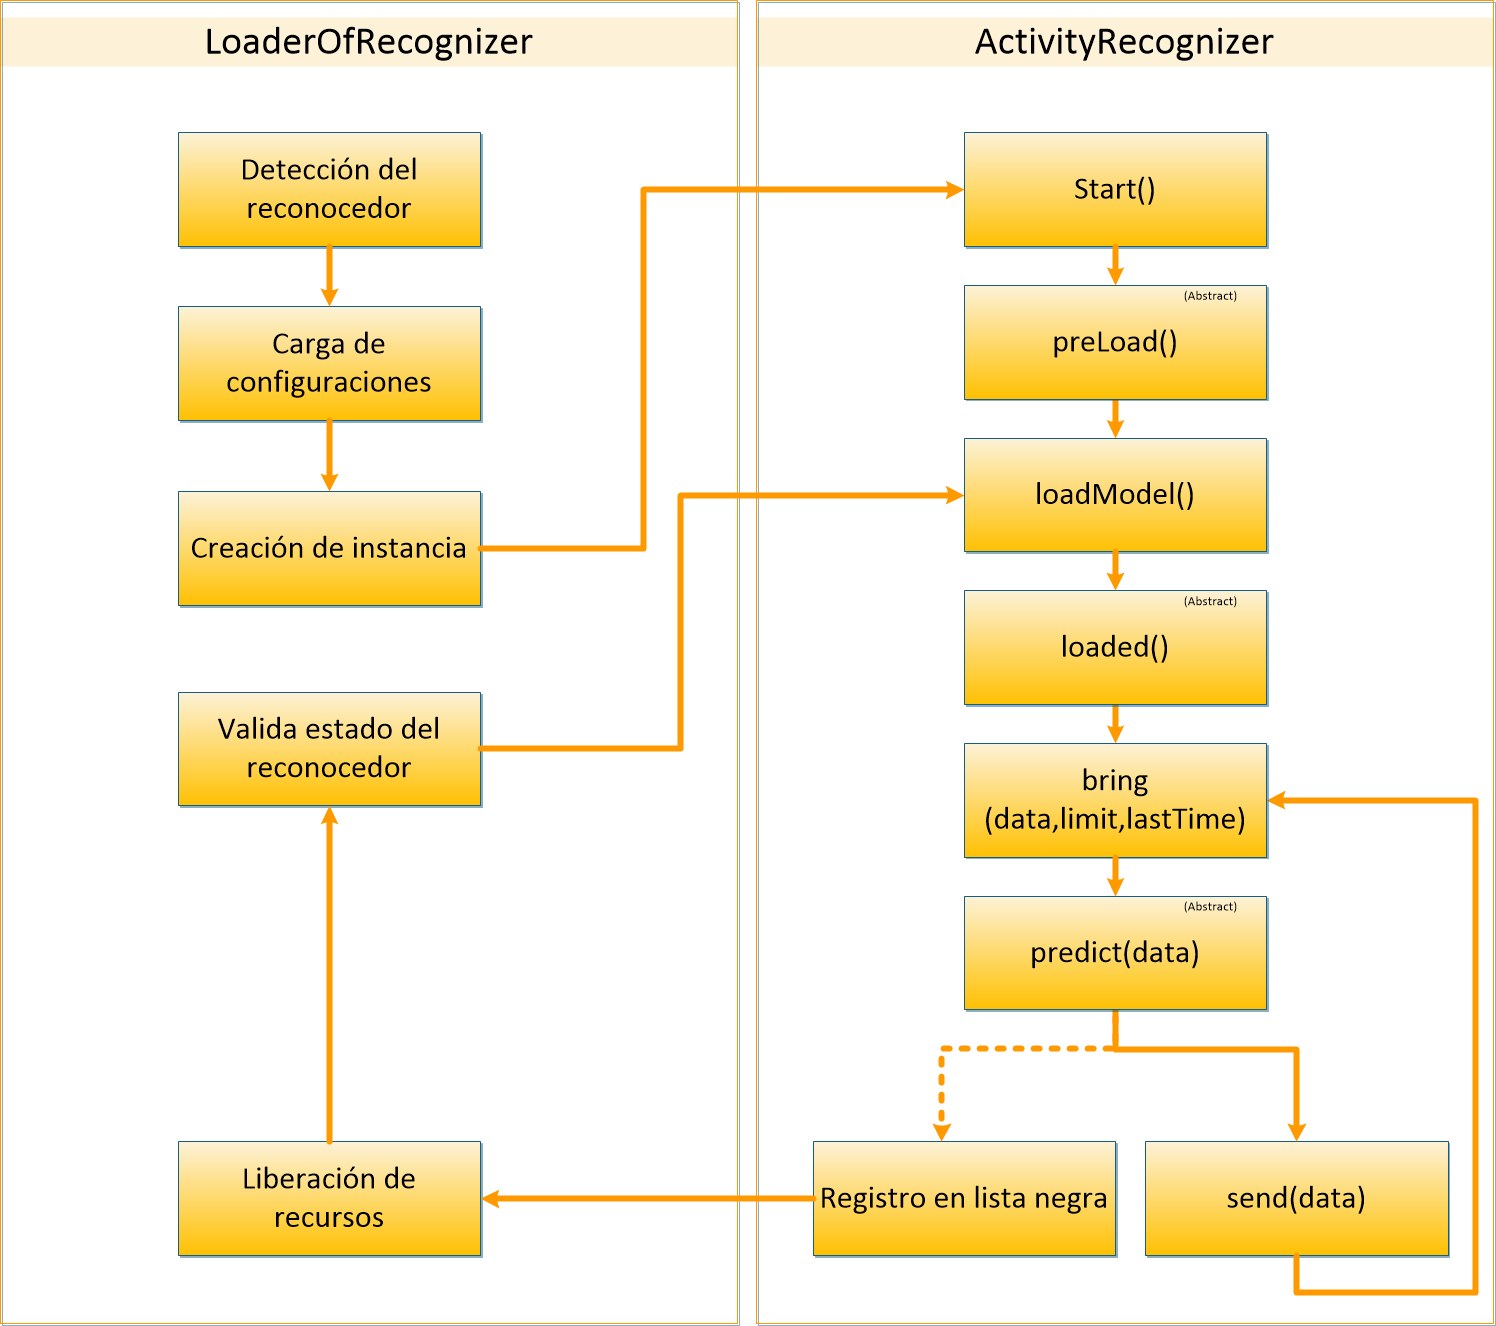
\includegraphics[width=0.9\linewidth]{imgs/03-Architecture/03-HARLifeCicle.png}
        	\caption[Ciclo de vida del proceso de reconocimiento de actividades]{Ciclo de vida del proceso de reconocimiento de actividades. A la izquierda las tareas realizadas por el cargador de reconocedores (LoaderOfRecognizer). A la derecha las tareas realizadas por el reconocedor de actividades (ActivityRecognizer).}
    	    \label{fig:HARLifeCicle}
        \end{figure}%
    
    Esta sección del sistema consta de dos artefactos principales: el cargador de reconocedores y el reconocedor de actividades (ver figura \ref{fig:HARLifeCicle}). Mediante la combinación de ambos se logra la detección de eventos particulares, como puede ser una persona sufriendo un infarto.
    
    \subsection{Cargador de reconocedores - LoaderOfRecognizer}
    \label{LoaderHAR}
        Esta clase se basa en definición del patrón ``método factoría'' y cumple tres funciones principales, primero identifica que reconocedores están disponibles para el reconocimiento de actividades, luego carga e inicia cada uno y por último se asegura que los se mantengan en funcionamiento.
        
        \subsubsection{Detección de reconocedores}
        \label{sub2:HARDetection}
            Esta tarea se lleva acabo cuando el cargador de reconocedores es inicializado y recorre la carpeta ``Recognizers'' en búsqueda de archivos con nombre ``config.yaml''. De esta forma, toda sub carpeta dentro de ``Recognizers'' que contenga un archivo de configuración, será considerado un posible componente a cargar.
            
            Como se mostró en la se sección \ref{Sec:ComponentStructure} cada componente debe contar con un archivo ``config.yaml'', el cual permitirá al cargador identificar características como la clase que debe ser inicializada para cargar el componente además de parámetros particulares.
            
            Para tomarlo como un componente válido, el archivo de configuración debe cumplir con los criterios expuestos en la sección \ref{Sec:ComponentStructure}, asegurando además que el estado del mismo esté asignado como ``Activo'' (Enabled). 
            
            Adicional a las variables generales de configuración, los componentes Reconocedores, en el archivo ``config.yaml'', cuentan con algunas variables adicionales: 
            
            \begin{itemize}
                \item \textbf{CLASSES}: Lista de eventos u objetos que puede reconocer el componente.
                \item \textbf{MODEL}: Ruta al archivo modelo del entrenamiento o conocimiento de la Inteligencia artificial \index{IA} que permitirá la inferencia.
                \item \textbf{FILTER\_NAME}: Nombre del controlador del cual se desea traer la información almacena en la pila de datos
                \item \textbf{FILTER\_ITEM}: Nombre del dispositivo que se desea consultar.
                \item \textbf{FILTER\_LIMIT}: Número de datos a consultar. -1 en caso de no requerir un límite de datos.
            \end{itemize}
            
        \subsubsection{Inicio de reconocedores}
        \label{sub2:HarStarting}
            Gracias al uso del patrón de 'método plantilla' (ver \ref{sub:FrameTemplateMethod}), el cargador de reconocedores es capaz de cargar de forma dinámica componentes que hayan sido creados en el momento que se desarrolla este sistema o posteriormente, incluso componentes que se pongan en la carpeta de ``Recognizers'' después de haber iniciado el sistema, siempre que cumpla con las características que se presentan en la sección de detección de reconocedores.
            
            Una vez cargado el Reconocedor, creado una instancia del mismo, se invocan el método \textit{start} implementado en la clase padre del componente (ver \ref{sub:ClassifierHAR}).En adelante, el componente será gestionado por la clase ``ActivityRecognizer'', salvo que se presenté algún error no controlado y éste se detenga, en cuyo caso el cargador de reconocedores intentará iniciarlo nuevamente.
        
        \subsubsection{Manteniendo reconocedores funcionando}
        \label{sub2:ClassifierKeepAlive}
            La naturaleza del sistema impone que todos sus componentes mantengan un funcionamiento constante incluso con la posibilidad de fallos. Si un reconocedor que detecte, por ejemplo, ``infartos'' presenta algún error, el cargador intentará volver a iniciar reconocedor, sin afectar el funcionamiento de los otros componentes que se ejecutan en el sistema ya que cada reconocedor se mantiene tiene aislado de los demás.
            
            Para ello, cuando un reconocedor, es registrado en una lista negra. El cargador de reconocedores, cada 30 segundos recorre el listado de reconocedores en lista negra (ver patrón iterador \ref{sub:FrameIterator}) e intenta volver a a iniciarlo. En caso de tener éxito, el reconocedor es retirado de la lista negra y estará listo nuevamente para consultar y a enviar datos a la pila.
            
            Adicionalmente, este componente es capaz, en cualquier momento y de forma automática, de detectar cambios en el archivo de configuración, recargando el reconocedor con sus nuevas configuraciones. 
    
    \subsection{reconocedor de actividades - ActivityRecongnizer}
    \label{sub:ClassifierHAR}
    
        Los componentes reconocedores, son los encargados de realizar la identificación de actividades humanas como tal. Estos componentes consultan y procesan, la información entregada por los dispositivos, para ellos pueden usar una o varias etapas de procesamiento, incluyendo técnicas de inteligencia artificial. Al finalizar el proceso informará, a la pila de datos, las actividades detectadas, además del identificador del dato en que fue detectado. 
    
        Cada componente Recognizer adherido al sistema cuenta con el aprendizaje necesario para las predicciones. Aunque este entrenamiento se hará al margen sistema, este trabajo provee tanto una plantilla para la creación de este tipo de componente que será presentado más adelante (sección \ref{Sec:ClassifierHARTemplate}), como conjuntos de datos y utilidades para realizar el entrenamiento de inteligencias artificiales, lo cual permitirá extender el sistema mediante la creación de nuevos componentes que identifiquen diferentes eventos o actividades humanas.
        
        Debido al diseño modular del sistema, cada componente reconocedor podrá ser ejecutado en máquinas independientes lo cual, además, se hace recomendable para asegurar la suficiente capacidad de procesamiento, puesto que los algoritmos que contienen estos componentes pueden requerir de procesamiento exhaustivo.
        
        El reconocedor de eventos se basa en la implementación de una clase abstracta (clase padre) que define las reglas para la construcción de un reconocedor de un evento específico. Cualquier reconocedor debe heredar de la clase abstracta ``ActivityRecongnizer'', obligándole a implementar algunos métodos específicos, aunque también se cuenta con algunos previamente implementados. Los siguientes métodos serán presentados siguiendo el ciclo de vida del proceso de reconocimiento de actividades en la figura \ref{fig:HARLifeCicle}. 
        
        \begin{itemize}
        
            %  --- start Recognizer
            \item \textbf{\textit{start}} (alg. \ref{Alg:startHAR}): 
            Inicia el módulo que realiza el reconocimiento de actividades con los datos alojados en la pila de datos.
            \begin{lstlisting}[language=Python, caption={Firma del método ``\textit{start}'' de la clase ActivityRecognizer.}, label=Alg:startHAR, numbers=none]
def start(self):
            \end{lstlisting}
            
            %  --- preLoad Recognizer
            \item \textbf{\textit{preLoad}} (alg. \ref{Alg:preLoadHAR}):
            (Abstracto) Método invocado antes de iniciar el procesamiento. Tiene el objetivo de permitir cargar los recursos necesarios del componente. También puede cambiar el valor de cualquier parámetro de configuración antes de los procesos automáticos, como puede ser el cambio de la ruta de la base de conocimiento. 
            \begin{lstlisting}[language=Python, caption={Firma del método ``\textit{preLoad}'' de la clase ActivityRecognizer.}, label=Alg:preLoadHAR, numbers=none]
@abc.abstractmethod
def preLoad(self):
            \end{lstlisting}
            
            %  --- loadModel Recognizer
            \item \textbf{\textit{loadModel}} (alg. \ref{Alg:loadModelHAR}):
            Una de las cualidades de los sistemas de inteligencia artificial es que los entrenamientos o base de conocimiento puede ser almacenada para utilizarla posteriormente. Esta función define el punto de carga de la base de conocimiento. La ruta de este conocimiento será obtenida del archivo de configuración del propio componente. 
            \begin{lstlisting}[language=Python, caption={Firma del método ``\textit{loadModel}'' de la clase ActivityRecognizer.}, label=Alg:loadModelHAR, numbers=none]
@abc.abstractmethod
def loadModel(self):

            \end{lstlisting}
            
            %  --- loaded Recognizer
            \item \textbf{\textit{loaded}} (alg. \ref{Alg:loadedHAR}):
            (Abstracto) Método invocado después de la carga de la base de conocimiento y tiene como fin la preparación o ajuste de los recursos necesarios antes de la predicción. También puede cambiar el valor de cualquier parámetro de configuración antes de la predicción. 
            \begin{lstlisting}[language=Python, caption={Firma del método ``\textit{loaded}'' de la clase ActivityRecognizer.}, label=Alg:loadedHAR, numbers=none]
@abc.abstractmethod
def loaded(self):
            \end{lstlisting}
            
            %  --- bring Recognizer
            \item \textbf{\textit{bring}} (alg. \ref{Alg:bringHAR}): 
            Consulta los datos disponibles en la pila. Recibe como parámetro los diferentes valores de filtrado que se adecuen a componente, esto es un objeto ``Data'', cuántos datos traer ('\textit{limit}') y el tiempo base de consulta ('\textit{lastTime}') para traer los datos más recientes.
            \begin{lstlisting}[language=Python, caption={Firma del método ``\textit{bring}'' de la clase ActivityRecognizer.}, label=Alg:bringHAR, numbers=none]
def bring(self, dataFilter:Data, limit=-1, lastTime=0):
            \end{lstlisting}
            
            %  --- predict Recognizer
            \item \textbf{\textit{predict}} (alg. \ref{Alg:predictHAR}):
            (Abastracto) Realiza la identificación de un evento en el dato recibido ('\textit{data}') y envía las clases detectadas y el identificador del dato a la pila.
            \begin{lstlisting}[language=Python, caption={Firma del método ``\textit{predict}'' de la clase ActivityRecognizer.}, label=Alg:predictHAR, numbers=none]
@abc.abstractmethod
def predict(self, data):
            \end{lstlisting}
            
            %  --- send Recognizer
            \item \textbf{\textit{send}} (alg. \ref{Alg:sendHAR}):
            Envía los datos de la detección ('\textit{idData}', '\textit{classes}') a la pila de datos.
            \begin{lstlisting}[language=Python, caption={Firma del método ``\textit{send}'' de la clase ActivityRecognizer.}, label=Alg:sendHAR, numbers=none]
def send(self, data:Data):
            \end{lstlisting}
            
            %  --- check Recognizer
            \item \textbf{\textit{check}} (alg. \ref{Alg:checkRecognizer}): 
            (abstracto) En caso de que reconocedor de actividades tenga algún problema y se detenga, se intentará liberar los recursos utilizados y validar nuevamente que los necesarios están disponibles.
            
            Este método retornara un valor de ``Verdadero'' o ``Falso'' inidcando si el componente puede ser reiniciado.
            
            \begin{lstlisting}[language=Python, caption={Firma del método ``\textit{check}'' de la clase ActivityRecognizer.}, label=Alg:checkRecognizer, numbers=none]
def check(self):
            \end{lstlisting}
        
        \end{itemize}
        
        Además de los métodos mencionados, la clase ``ActivityRecognizer'' espera la implementación de algunos métodos adicionales.
        
        \begin{itemize}
            
            %  --- showData Controller
            \item \textbf{\textit{showData}} (alg. \ref{Alg:showDataHAR}):
            (Abstracto) Este método es útil para presentar los resultados del procesamiento e inferencia de eventos, cuando el componente inicia de forma independiente. Este método será invocado en lugar del método \textbf{\textit{send}}.
            \begin{lstlisting}[language=Python, caption={Firma del método ``\textit{showData}'' de la clase ActivityRecognizer.}, label=Alg:showDataHAR, numbers=none]
@abc.abstractmethod
def showData(self, dataPredicted, dataSource):
            \end{lstlisting}
            
            %  --- Simulate Recognizer
            \item \textbf{\textit{simulateData}} (alg. \ref{Alg:simulateRecognizer}):
            (Abstracto) Este método es útil para simular la consulta en la pila de datos, cuando el componente inicia de forma independiente. Este método será invocado en lugar del método \textbf{\textit{bring}}. Esto permitirá no depender de los controladores de dispositivos, además que facilita las pruebas del componente en estado de desarrollo.
            \begin{lstlisting}[language=Python, caption={Firma del método ``\textit{simulateData}''.}, label=Alg:simulateRecognizer, numbers=none]
@abc.abstractmethod
def simulateData(self,data:Data, limit:int=-1, lastTime:float=-1):
            \end{lstlisting}
            
            %  --- stop recognizer
            \item \textbf{\textit{stop}} (alg. \ref{Alg:stopHAR}):
            (Abstracto) Detiene la ejecición el componente. 
            \begin{lstlisting}[language=Python, caption={Firma del método ``\textit{stop}''.}, label=Alg:stopHAR, numbers=none]
def stop(self):
            \end{lstlisting}
            
        \end{itemize}
    
    \newpage

\section{Sección C - Analizador de eventos y notificación de alertas}
\label{Sec:Analyzer}
    En esta sección del sistema se encuentran los componentes encargados de analizar los eventos simples detectados por los diferentes componentes Analizadores de eventos y de notificación. Siendo éstas las piezas finales para emitir notificaciones sobre la anormalidad detectada (ver fig. \ref{fig:Architecture}).
    
        \begin{figure}[ht!]
        	\centering
        	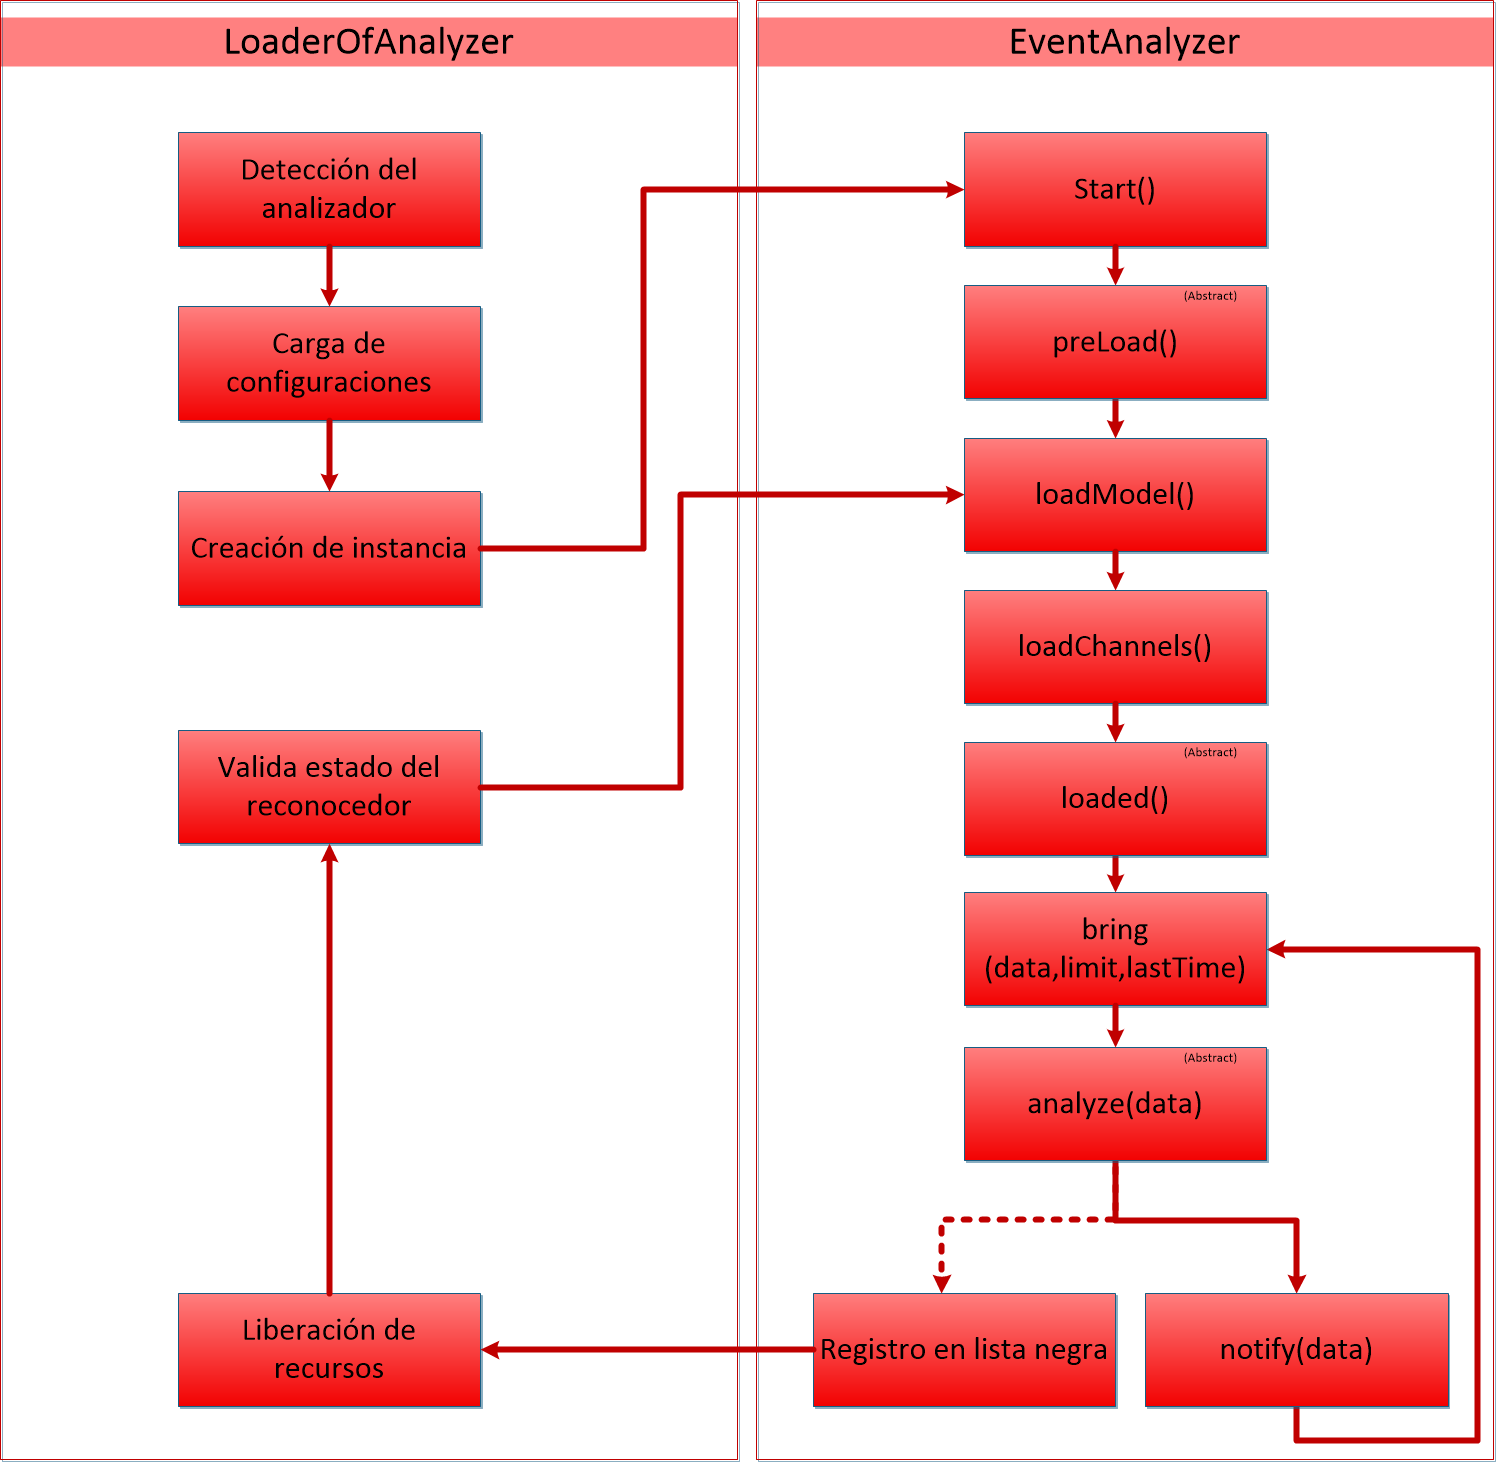
\includegraphics[width=0.9\linewidth]{imgs/03-Architecture/03-AnalyzerLifeCicle.png}
        	\caption[Ciclo de vida del análisis de eventos]{Ciclo de vida del análisis de eventos. A la izquierda las tareas realizadas por el cargador de analizadores (LoaderOfAnalyzer). A la derecha las tareas realizadas por el analizador de eventos (EventAnalyzer).}
    	    \label{fig:AnalyzerLifeCicle}
        \end{figure}%
    
    Al igual que los componentes, Controlador de dispositivos y Reconocedor de actividades, El Analizador de Eventos (``Event Analyzer'' \index{Event Analyzer}) puede ejecutarse de forma independiente, es decir que permite su ejecución simultanea en múltiples ordenadores. 
    
    Por otro lado, el Canal de notificación (``Channel''\index{Channel}) solo está pensado como un medio de comunicación de los eventos que el Analizador requiera informar. De esta forma, un Canal de notificación solo se ejecutara a petición de otro componente. Cuando un analizador de eventos identifique una anomalía, éste iniciará los notificadores disponibles, por tanto, los componentes de notificación deben estar en el mismo ordenador que el analizador (ver figura \ref{fig:AnalyzerLifeCicle}).
    
    A continuación serán presentados los artefactos que componen tanto el Analizador de Eventos como el Canal de notificaciones. De igual manera será presentada una plantilla, provista en este mismo trabajo, para la creación de este tipo de componentes (ver secciones \ref{Sec:EventAnalyzerTemplate} y \ref{Sec:NotifierChannelTemplate}).
    
    \subsection{Cargador de Analizadores - LoaderAnalyzer}
    \label{sub:LoaderAnalyzer}
        De forma similar a los componentes de las secciones anteriores del sistema, el componente Analizador de Eventos cuenta con dos artefactos que permiten, por un lado, su continuo funcionamiento y por otro la identificación de los eventos anómalos. El primero de ellos es el Cargador de Analizadores.
    
        Este componente cumple tres funciones principales, primero identifica que analizadores están disponibles para la identificación de eventos anómalos, luego carga e inicia cada uno y, por último, se asegura que los componentes iniciados se mantengan en ejecución o de ser necesario, volverlos a iniciar.
        
        \subsubsection{Detección de analizadores}
        \label{sub2:AnalyzerDetection}
            Esta acción ocurre cuando el cargador de analizadores es inicializado y recorre la carpeta 'Analyzers' en búsqueda de archivos con nombre 'config.yaml'. De esta forma, toda sub carpeta dentro de ``Analyzers'' que contenga un archivo de configuración, será considerado un posible componente a cargar,
            
            Como se mostró en la se sección \ref{Sec:ComponentStructure} cada componente debe contar con un archivo 'config.yaml', el cual permitirá al cargador identificar las variables de configuración necesarias para el funcionamiento de los componentes.
            
            Para tomarlo como un componente válido, el archivo de configuración debe cumplir con los criterios expuestos en la sección \ref{Sec:ComponentStructure}, asegurando además que el estado del mismo esté asignado como ``Activo'' (Enabled). 
            
            Adicional a las variables generales de configuración, los componentes Analizadores, en el archivo ``config.yaml'', cuentan con algunas variables adicionales: 
            
            \begin{itemize}
                \item \textbf{CLASSES}: Lista de eventos u objetos que puede reconocer el componente.
                \item \textbf{MODEL}: Ruta al archivo modelo del entrenamiento o conocimiento de la Inteligencia artificial \index{IA} que permitirá la inferencia.
                \item \textbf{FILTER\_NAME}: Nombre del Reconocedor del cual se desea traer la información almacena en la pila de datos
                \item \textbf{FILTER\_ITEM}: Sub Nombre del reconocedor que se desea consultar.
                \item \textbf{FILTER\_LIMIT}: Número de datos a consultar. -1 en caso de no requerir un límite de datos.
            \end{itemize}
        
        \subsubsection{Inicio de analizadores}
        \label{sub2:AnalyzerStarting}
            Gracias al uso del patrón de 'método plantilla' (ver \ref{sub:FrameTemplateMethod}), el cargador de analizadores es capaz de cargar de forma dinámica componentes, hayan sido creados en el momento que se desarrolla este sistema o posteriormente, incluso componentes que se pongan en la carpeta de ``Analyzers'' después de haber iniciado el sistema, siempre que cumpla con las características que se presentan en la sección de detección de analizadores.
            
            Una vez cargado el Analizador, creado una instancia del mismo, se invoca el método \textit{start} implementado en la clase padre del componente (ver \ref{sub:EventAnalyzer}). Posteriormente el método \textit{start} ira cargando los métodos sucesivos del ciclo de vida del análisis de eventos como se muestra en la figura \ref{fig:AnalyzerLifeCicle}. En adelante, el componente será gestionado por la clase ``ActivityRecognizer'', salvo que se presenté algún error no controlado y éste se detenga, en cuyo caso el cargador de reconocedores intentará iniciarlo nuevamente.
        
        \subsubsection{Manteniendo Analizadores funcionando}
        \label{sub2:AnalyzerKeepAlive}
            La naturaleza del sistema impone que todos sus componentes mantengan un funcionamiento constante incluso con la posibilidad de fallos. De esta forma, si un componente de este tipo presenta algún error no controlado que obligue su detención, el Cargador de Analizadores intentará volver a cargarlo e iniciarlo, sin afectar el funcionamiento de los otros componentes que se ejecutan en el sistema ya que cada componente se mantiene tiene aislado de los demás.
            
            Para ello, cuando un analizador falla y se detiene su ejecución, es registrado en una lista negra. El cargador de analizadores, cada 30 segundos recorre el listado de analizadores en lista negra (ver patrón iterador \ref{sub:FrameIterator}) e intenta volver a iniciarlo. Para ello se liberan los recursos cargados en memoria, como es el caso de la base de conocimiento, y se verifica que los recursos necesarios están disponibles, luego de esto el analizador es retirado de la lista negra y estará listo nuevamente para consultar analizar los eventos registrados en la pila de datos.
            
            Adicionalmente, este componente es capaz, en cualquier momento y de forma automática, de detectar cambios en el archivo de configuración, recargando el componente con sus nuevas configuraciones.
            
    \subsection{Analizador de eventos - EventAnalyzer}
    \label{sub:EventAnalyzer}
        Los componentes analizadores, son los encargados de realizar la interpretación de los eventos detectados por los Reconocedores de actividades. Estos componentes pueden consultar las etiquetas generadas por los Reconocedores y entregadas por la pila de datos en forma de frases cortas tipo: 
        
        \begin{itemize}
            \item At $<\textbf{Hora}>$ the $<\textbf{Componente}>$ detect $<\textbf{Eventos}>$ in $<\textbf{Nombre del dispositivo}>$ of $<\textbf{Controlador}>$.".
        \end{itemize}
        
        Por ejemplo:
        
        \begin{itemize}
            \item At \textbf{14:00} the \textbf{InfarctSkeleton} detect \textbf{``Infarct''} in \textbf{livingRoom1} of \textbf{CamController}.".
        \end{itemize}
        
        %https://relopezbriega.github.io/blog/2017/09/23/procesamiento-del-lenguaje-natural-con-python/
        
        De esta forma, apoyándose en técnicas de procesamiento de lenguaje natura (PLN\index{PLN}), es capaz de interpretar las frases consultadas, como si de un narrador se tratara, y generando alertas cuando una anormalidad sea detectada en las frases. Por ejemplo, el sistema reportara una persona tirada en el suelo todos los días a la misma hora, el sistema lo entenderá como un comportamiento habitual, sin embargo, si el sistema nunca reportó este comportamiento podría generar una alerta e invocar a los canales de notificaciones.
        
        El componente analizador de eventos se basa en la implementación de una clase abstracta (clase padre) que define las reglas para la construcción de nuevos analizadores. Cualquier componente analizador debe heredar de la clase abstracta ``\textbf{EventAnalyzer}'', obligándole a implementar algunos métodos específicos, aunque también se cuenta con algunos previamente implementados. Los siguientes métodos serán presentados siguiendo el ciclo de vida del proceso de análisis de actividades mostrado en la figura \ref{fig:AnalyzerLifeCicle}.

        \begin{itemize}
        
            %  --- Start Analyzer
            \item \textbf{\textit{start}} (alg. \ref{Alg:startAnalyzer}): 
            Inicia el módulo para empezar a analizar los eventos reportados. Así mismo, este método ejecuta los métodos subsecuentes del ciclo de análisis de eventos.
            \begin{lstlisting}[language=Python, caption={Firma del método "\textit{start}" de la clase EventAnalyzer.}, label=Alg:startAnalyzer, numbers=none]
def start(self):
            \end{lstlisting}
            
            %  --- preLoad Analyzer
            \item \textbf{\textit{preLoad}} (alg. \ref{Alg:preLoadAnalyzer}):
            (Abstracto) Método invocado antes de iniciar el procesamiento. Tiene el objetivo de cargar los recursos necesarios para el componente o reasignar los parámetros de configuración previó a la ejecución de análisis o carga de canales de notificación.
            \begin{lstlisting}[language=Python, caption={Firma del método "\textit{preLoad}" de la clase EventAnalyzer.}, label=Alg:preLoadAnalyzer, numbers=none]
@abc.abstractmethod
def preLoad(self):
            \end{lstlisting}
            
            %  --- loadModel Analyzer
            \item \textbf{\textit{loadModel}} (alg. \ref{Alg:loadModelAnalyzer}):
            Una de las cualidades de los sistemas de inteligencia artificial es que los entrenamientos o base de conocimiento puede ser almacenada para utilizarla posteriormente. Esta función define el punto de carga de la base de conocimiento. La ruta de este conocimiento será obtenida del archivo de configuración del propio componente. 
            \begin{lstlisting}[language=Python, caption={Firma del método "\textit{loadModel}" de la clase EventAnalyzer.}, label=Alg:loadModelAnalyzer, numbers=none]
@abc.abstractmethod
def loadModel(self):
            \end{lstlisting}
            
            %  --- loadChannels Analyzer
            \item \textbf{\textit{loadChannels}} (alg. \ref{Alg:loadChannelsAnalyzer}):
            Identifica los componentes notificadores disponibles y los carga para su uso posterior, de está forma la invocación se hará más rápidamente.
            \begin{lstlisting}[language=Python, caption={Firma del método "\textit{loadChannels}" de la clase EventAnalyzer.}, label=Alg:loadChannelsAnalyzer, numbers=none]
def loadChannels(self):
            \end{lstlisting}
            
            %  --- loaded Analyzer
            \item \textbf{\textit{loaded}} (alg. \ref{Alg:loadedAnalyzer}):
            (Abstracto) Método invocado después de la carga de la base de conocimiento y los canales de notificación. Tiene como fin la preparación o ajuste de los recursos necesarios antes del análisis de los eventos.
            \begin{lstlisting}[language=Python, caption={Firma del método ``\textit{loaded}'' de la clase EventAnalyzer.}, label=Alg:loadedAnalyzer, numbers=none]
@abc.abstractmethod
def loaded(self):
            \end{lstlisting}
            
            %  --- bring Analyzer
            \item \textbf{\textit{bring}} (alg. \ref{Alg:bringAnalyzer}):
            Consulta los eventos reportados a la pila. Recibe como parámetro los diferentes valores de filtrado que se adecuen a componente, esto es un objeto ``Data'', cuántos datos traer ('\textit{limit}') y el tiempo base de consulta ('\textit{lastTime}') para traer los datos más recientes.
            \begin{lstlisting}[language=Python, caption={Firma del método "\textit{bring}" de la clase EventAnalyzer.}, label=Alg:bringAnalyzer, numbers=none]
def bring(self, data, limit=-1, lastTime=0):
            \end{lstlisting}
            
            %  --- analyze Analyzer
            \item \textbf{\textit{analyze}} (alg. \ref{Alg:analyzeAnalyzer}):
            (Abstracto) Realiza el análisis de los eventos detectados por los reconocedores de actividad. En caso de identificar uno o un conjunto de eventos que deban ser notificados, invocará el método de notificación y emitirá el mensaje por todos los canales dispuestos.
            \begin{lstlisting}[language=Python, caption={Firma del método "\textit{analyze}" de la clase EventAnalyzer.}, label=Alg:analyzeAnalyzer, numbers=none]
@abc.abstractmethod
def analyze(self, data):
            \end{lstlisting}
            
            %  --- notify Analyzer
            \item \textbf{\textit{notify}} (alg. \ref{Alg:notifyAnalyzer}):
            Envía un mensaje a los notificadores para que transmitan el mensaje por los canales disponibles. Los notificadores pueden ser de diferentes tipos, como se presentará más adelante, incluyendo envío de correo, sms, presentación de datos, el informe a la pila de datos de la anormalidad o el resguardo de los datos donde la anormalidad se detectó.
            \begin{lstlisting}[language=Python, caption={Firma del método "\textit{notify}" de la clase EventAnalyzer.}, label=Alg:notifyAnalyzer, numbers=none]
def notify(self, data):
            \end{lstlisting}
            
            %  --- check Analyzer
            \item \textbf{\textit{check}} (alg. \ref{Alg:checkAnalyzer}): 
            (abstracto) En caso de que el analizador tenga algún problema y se detenga, se intentará comprobar con esta función, liberar los recursos utilizados y validar que los necesarios, según el archivo de configuración, están disponibles para su uso.
            
            Este método retornara un valor de ``Verdadero'' o ``Falso'' indicando el componente puede ser cargado nuevamente.
            
            \begin{lstlisting}[language=Python, caption={Firma del método ``\textit{check}'' de la clase ActivityRecognizer.}, label=Alg:checkAnalyzer, numbers=none]
def check(self):
            \end{lstlisting}
            
        \end{itemize}
        
        Adicional a los métodos presentados, la clase ``\textbf{EventAnalyzer}'', espera la implementación de algunos métodos adicionales.
        
        \begin{itemize}
            
            %  --- showData analyzer
            \item \textbf{\textit{showData}} (alg. \ref{Alg:showDataAnalyzer}):
            (Abstracto) Este método es útil para presentar los resultados del procesamiento e inferencia de eventos, cuando el componente inicia de forma independiente. Este método será invocado en lugar del método \textbf{\textit{notify}}.
            \begin{lstlisting}[language=Python, caption={Firma del método ``\textit{showData}'' de la clase EventAnalyzer.}, label=Alg:showDataAnalyzer, numbers=none]
@abc.abstractmethod
def showData(self, dataPredicted, dataSource):
            \end{lstlisting}
            
            %  --- Simulate Analyzer
            \item \textbf{\textit{simulateData}} (alg. \ref{Alg:simulateAnalyzer}):
            (Abstracto) Este método es útil para simular la consulta en la pila de datos, cuando el componente inicia de forma independiente. Este método será invocado en lugar del método \textbf{\textit{bring}}. Esto permitirá no depender de los reconocedores, además que facilita las pruebas del componente en estado de desarrollo.
            \begin{lstlisting}[language=Python, caption={Firma del método ``\textit{simulateData}''.}, label=Alg:simulateAnalyzer, numbers=none]
@abc.abstractmethod
def simulateData(self):
            \end{lstlisting}
            
            %  --- stop Analyzer
            \item \textbf{\textit{stop}} (alg. \ref{Alg:stopAnalyzer}): (Abstracto) Detiene la ejecución del componente. 
            \begin{lstlisting}[language=Python, caption={Firma del método "\textit{stop}" de la clase EventAnalyzer.}, label=Alg:stopAnalyzer, numbers=none]
def stop(self):
            \end{lstlisting}
            
        \end{itemize}
    
    \subsection{Canales de notificación - CommChannel}
    \label{sub:CommChannel}
        
        El segundo tipo componente de la sección C del sistema son los canales de notificación o simplemente notificadores. Estos se encargan de transmitir mensajes con las alertas detectadas por los analizadores, por ejemplo, una persona en el suelo o una persona con infarto.
        
        Cuando un componente Analizador de Eventos es iniciado, éste llamará a su vez al Cargador de Canales de Notificación (``LoaderOfChannel''). El cargador de Canales identifica los componentes disponibles para el envío de notificaciones y los mantendrá en memoria para agilizar la ejecución posterior.
        
        La extensión de nuevos canales de notificación, consisten en la implementación de una clase abstracta (clase padre: ``NotificationChannel''), que permitirá enviar mensajes por diferentes canales, por ejemplo, correo electrónico, SMS, Redes sociales, Apps móvil o cualquier otro canal de comunicación que se desee. 
        
        La arquitectura del sistema permite que, usando una plantilla provista en este trabajo (ver sección \ref{Sec:NotifierChannelTemplate}), se puedan crear nuevos módulos de este tipo para, así, dar una mayor escalabilidad al sistema, permitiendo a futuro adicionar nuevos medios de comunicación. Aunque se aclara que para la demostración de este tipo de componentes solo se han creados dos componentes notificadores uno para correo electrónico y otro para notificación directa a una APP móvil. 
    
        \begin{figure}[ht!]
        	\centering
        	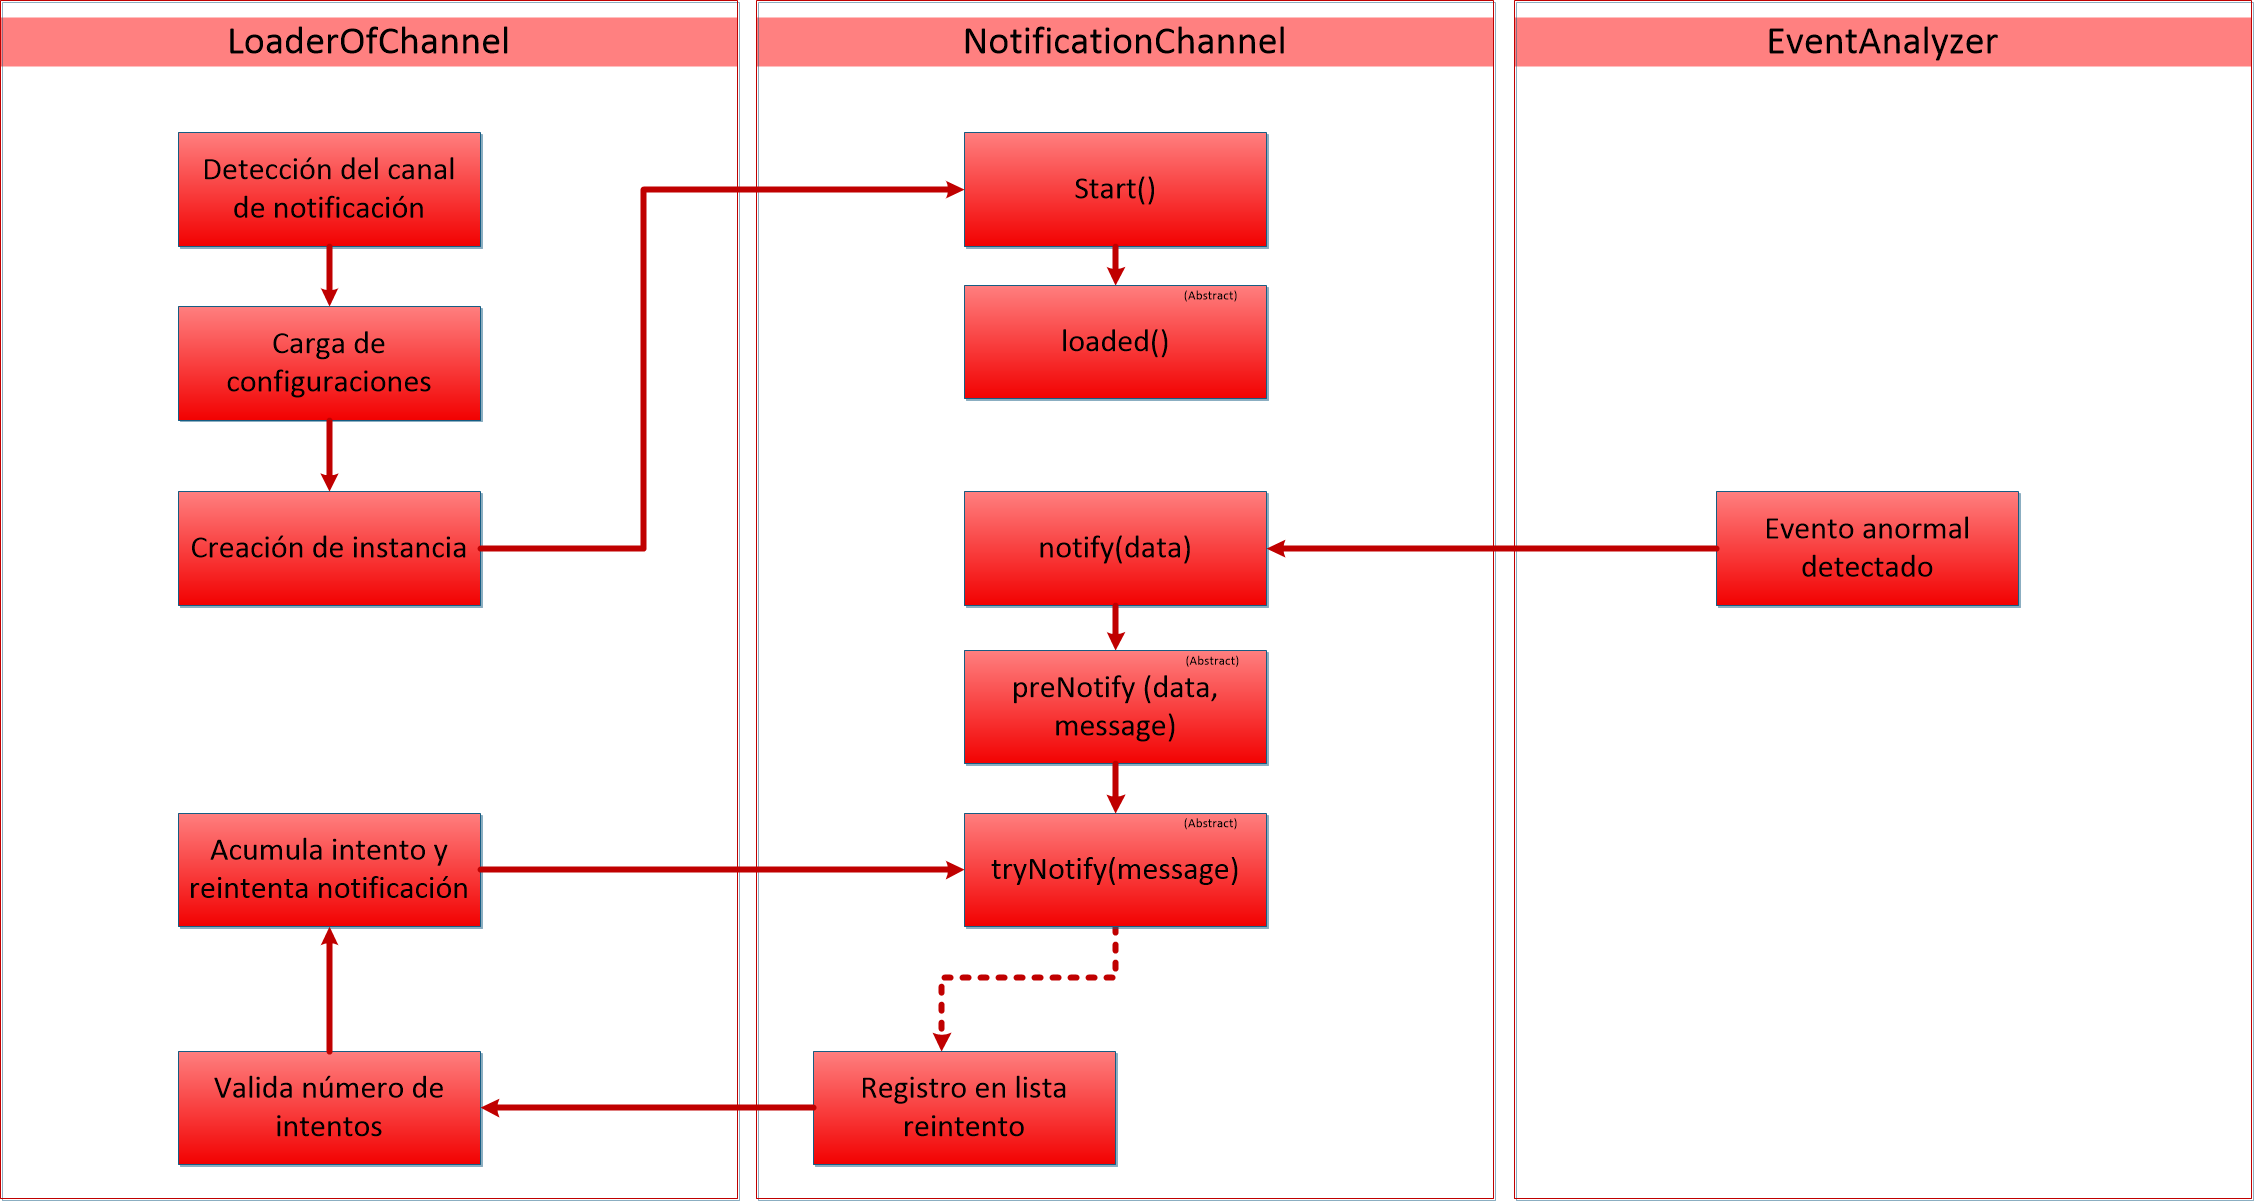
\includegraphics[width=0.9\linewidth]{imgs/03-Architecture/03-NotifyLifeCicle.png}
        	\caption[Ciclo de vida de una notificación]{Ciclo de vida de una notificación. A la izquierda las tareas realizadas por el cargador de canales de notificación (LoaderOfChannel). Al centro las tareas realizadas por el canal de notificación (NotificationChannel). Al derecha las tareas realizadas por el analizador de eventos (EventAnalyzer).}
    	    \label{fig:NotifyLifeCicle}
        \end{figure}%
        
        De forma similar a los demás componentes ya presentados, la notificación también tiene un ciclo de vida propio, como se muestra en la figura \ref{fig:NotifyLifeCicle}. Dado que cualquier componente notificador debe heredar de la clase abstracta ``\textbf{NotificationChannel}'', se obliga a implementar algunos métodos específicos, aunque también se cuenta con algunos previamente implementados. Los siguientes métodos serán presentados siguiendo el ciclo de vida de una notificación mostrado en la figura \ref{fig:NotifyLifeCicle}.
    
        \begin{itemize}
        
            %  --- Start notifier
            \item \textbf{\textit{start}} (alg. \ref{Alg:startChannel}): 
            Inicializa y mantiene en memoria el canal de notificación.
            \begin{lstlisting}[language=Python, caption={Firma del método "\textit{start}" de la clase NotificationChannel.}, label=Alg:startChannel, numbers=none]
def start(self):
            \end{lstlisting}
            
            %  --- loaded notifier
            \item \textbf{\textit{preLoad}} (alg. \ref{Alg:loadedChannel}):
            (Abstracto) Método invocado una vez cargado en memoria el canal de notificación. Tiene el objetivo de cargar los recursos necesarios para el componente o reasignar los parámetros de configuración previó a la ejecución de de las notificaciones.
            \begin{lstlisting}[language=Python, caption={Firma del método "\textit{loaded}" de la clase NotificationChannel.}, label=Alg:loadedChannel, numbers=none]
@abc.abstractmethod
def loaded(self):
            \end{lstlisting}
        
            %  --- notify notifier
            \item \textbf{\textit{notify}} (alg. \ref{Alg:sendNotifier}):
            Este método recibe, por parte del componente Analizador de Eventos, la orden de envío de una notificación. Esta función recibirá los datos de la notificación y con esto se construirá un objeto tipo ``\textbf{Message}'' para posteriormente realizar el intento de notificación.
            \begin{lstlisting}[language=Python, caption={Firma del método "\textit{notify}" de la clase NotificationChannel.}, label=Alg:sendNotifier, numbers=none]
def notify(self, data):
            \end{lstlisting}
            
            %  --- preNotify notifier
            \item \textbf{\textit{preNotify}} (alg. \ref{Alg:preNotify}):
            (Abstracto) Este método permite la información necesaria para la construcción del mensaje, consultando, de ser necesario, información de la pila de datos. Esta función recibirá tanto los datos de la notificación como el el mensaje construido.
            \begin{lstlisting}[language=Python, caption={Firma del método "\textit{preNotify}" de la clase NotificationChannel.}, label=Alg:preNotify, numbers=none]
@abc.abstractmethod
def preNotify(self, data, message):
            \end{lstlisting}
            
            %  --- tryNotify notifier
            \item \textbf{\textit{tryNotify}} (alg. \ref{Alg:tryNotify}):
            (Abstracto) Este método realiza el envío del mensaje. En caso de fallar se agregará a una lista de reintentos que gestiona la clase ``\textbf{LoaderOfChannel}''
            \begin{lstlisting}[language=Python, caption={Firma del método "\textit{tryNotify}" de la clase NotificationChannel.}, label=Alg:tryNotify, numbers=none]
@abc.abstractmethod
def tryNotify(self, message):
            \end{lstlisting}
            
        \end{itemize}
        
    \subsection{Estructura de mensajes de notificación - Message}
    \label{sub:NotifyMessage}        
         La clase \textbf{\textit{Message}} define la estructura del objeto que será usado por los notificadores para construir el mensaje a enviar. La tabla \ref{Tab:MessageEstructureAttr} muestra los atributos que componen la clase \textbf{\textit{Data}}.
        
        \begin{table}[ht!]
        \caption[Atributos del mensaje a transmitir por los canales de notificación]{Atributos del mensaje a transmitir por los canales de notificación.}
        \label{Tab:MessageEstructureAttr}
        \centering
        \begin{tabular}{ | l p{11cm} | } 
            \hline
             \textbf{Atributo}  & \textbf{Descripción} \\ 
            \hline\hline
            \textbf{born}       & Fecha y hora de generación del mensaje. \\
            \hline
            \textbf{from*}      & Remitente del mensaje. \\
            \hline
            \textbf{to*}        & Lista de destinatarios. \\
            \hline
            \textbf{cc*}        & Lista de destinatarios en copia. \\
            \hline
            \textbf{bcc*}       & Lista de destinatarios en copia oculta o independiente. \\
            \hline
            \textbf{subject}    & Título del mensaje. \\
            \hline
            \textbf{message}    & Cuerpo del mensaje. \\
            \hline
            \textbf{aux}        & Permite almacenar información adicional, como la forma en que se organizan los datos o cualquier otro dato a conveniencia. \\
            \hline
        \end{tabular}
        * En caso de ir vacío lo tomara del archivo de configuración del componente.
        \end{table}
        
        \subsubsection{Variables de reemplazo en mensajes de notificación}
        \label{sub2:MessageTokens}
            Además de los atributos mencionados, es importante resaltar que todos los atributos, excepto '\textbf{born}', serán pasados por un reemplazador de tokens, lo cual permitirá el oso de palabras claves para su posterior reemplazo por los valores de contexto. Las palabras clave (tokens) disponibles son:
        
            \begin{itemize}
                \item \textbf{Controllers}: Controladores donde se originaron los datos que dieron lugar a la notificación.
                \item \textbf{Devices}: Dispositivos donde se originaron los datos que dieron lugar a la notificación.
                \item \textbf{Recognizers}: Reconocedores donde se identificaron los eventos que dieron lugar a la notificación.
                \item \textbf{Analyzer}: Analizadores donde se identificaron los eventos que dieron lugar a la notificación.
                \item \textbf{Events}: Eventos identificados por el Reconocedor.
                \item \textbf{DataControllersID}: Identificador de los datos recibidos desde los Controladores.
                \item \textbf{DataRecognizersID}: Identificador de los datos recibidos desde los Reconocedores.
                \item \textbf{DataAnalyzersID}: Identificador de los datos recibidos desde los Analizadores.
                \item \textbf{Phrases}: Frases utilizadas por el Analizador que dieron lugar a la notificación.
                \item \textbf{time}: Fecha y hora de generación del mensaje.
            \end{itemize}
        
    \newpage

\section{Modelo integrado del sistema}
\label{sec:IntegratedModel}
    Una vez presentadas las diferentes piezas del sistema es posible visualizar de forma integrada todos los componentes. Para ello serán presentados tres especificaciones que detallan la disposición e integración de las partes: Estructura de directorios, Modelo de clases y modelo de despliegue.
        
    \subsection{Estructura de directorios}
    \label{sub:Directories}
        Así como se definen los diferentes componentes y sus funcionalidades, este trabajo define de forma rígida la ubicación de los componentes. La figura \ref{fig:SystemDirectories} presenta el árbol de directorios agrupando los componentes en dos tipos: del núcleo y código base, por un lado, y componentes extensibles por el otro.
        
        \begin{figure}[ht!]
        	\centering
        	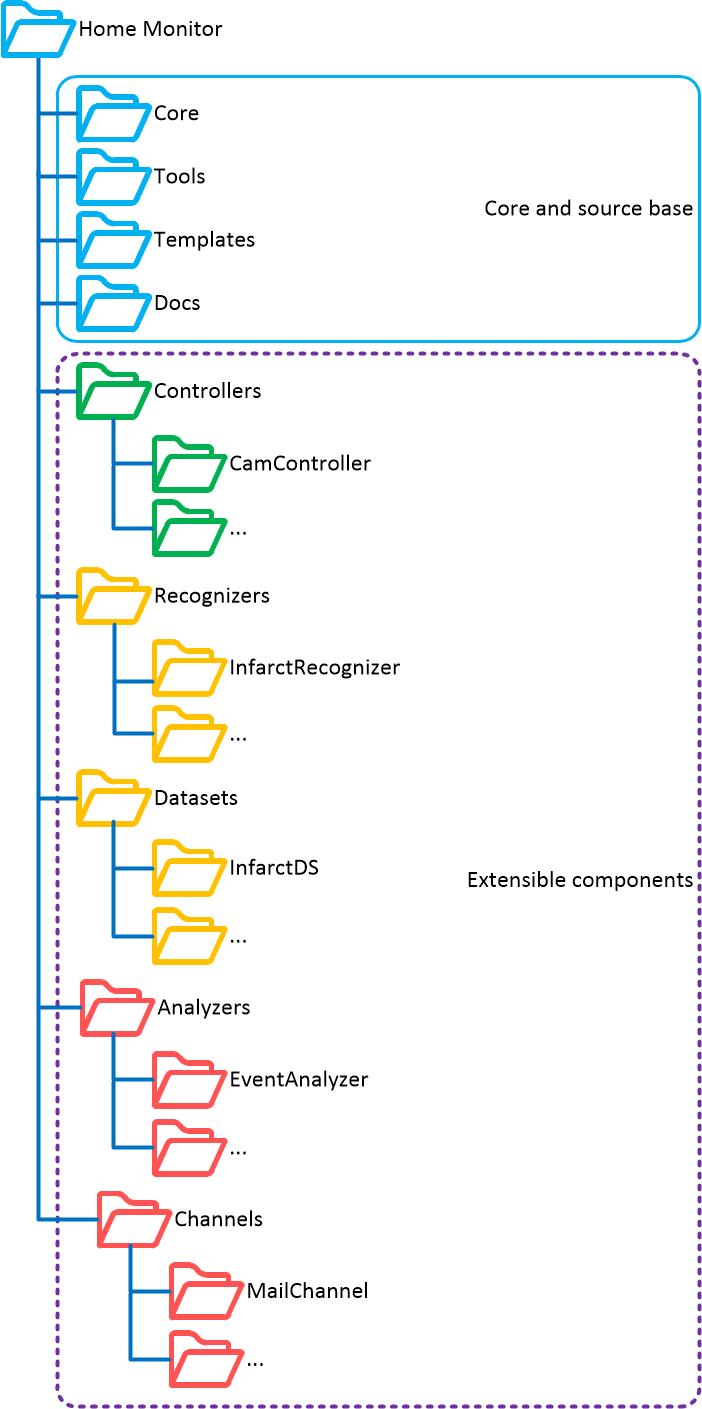
\includegraphics[width=0.5\linewidth]{imgs/03-Architecture/03-Directories.png}
        	\caption[Árbol de directorios]{Árbol de directorios. Presenta la ubicación en que debe ir cada uno de los componentes del sistema. En azul (arriba) las piezas del núcleo del sistema, en el recuadro morado (abajo) los componentes extensibles con funcionalidades específicas.}
    	    \label{fig:SystemDirectories}
        \end{figure}%
    
        \subsubsection{Núcleo y código base}
        \label{sub2:CoreBaseDirectories}
        
            Todas las piezas de software que componen el segmento de núcleo y código base se caracterizan por mantenerse rígidos en su definición y programación, asegurando la estabilidad del mismo, manteniendo principalmente un modelo de comunicación inmutable. Aunque el sistema es altamente escalable, esa escalabilidad se sustenta en la estabilidad y definición estática de este segmento del sistema. Los artefacto de este segmento se dividen en cuatro categorías: Directorio de componentes del núcleo (core), Directorio de herramientas (Tools), Directorio de plantillas (Templates), Directorio de documentación (Docs).
            
            \textbf{Directorio de componentes del núcleo}
            
                En este directorio se encuentran las clases más importantes del sistema. Es aquí donde se define la estructura del sistema y los mecanismos de aislamiento y comunicación de todos los demás componentes integrados al sistema. 
                
                \textcolor{red}{Listar las clases de la carpeta core}.
                
                Para empezar, aquí se encuentran los cargadores de componentes, estos se encargarán de iniciar y mantener funcionando todos los componentes del sistemas. Existe un cargador por cada tipo de componente y trabajan en conjunto con las clases padre de cada tipo de componente, de la cual heredaran cada nuevo componente que se agregue al sistema. Las clases padre, son la base fundamental de la homogeneidad del los componentes, pues aseguran una estructura igual, tanto en la programación como en el intercambio de información ya que proveen los métodos necesarios para el envío y solicitud de datos a la pila de datos.
                
                Además de lo mencionado, en este directorio se encuentra la implementación de la pila de datos, columna vertebral para el envío y transmisión de datos entre componentes.
                
                Finalmente, la clase 'main' que permite la carga del sistema en general.
            
            \textbf{Directorio de herramientas}
            
                En este directorio se encuentran piezas de software con funcionalidades generales, pero también clases enteras que facilitan el proceso de construcción de nuevos componentes o incluso la preparación de conjuntos de datos para entrenamientos. Las funcionalidades serán detalladas más adelante (ver secciones \ref{Sec:TrainValTestDataset} y \ref{Sec:Tools}).
            
            \textbf{Directorio de plantillas}
                
                La flexibilidad para que un sistema sea escalable depende, en gran medida, de la definición de estructuras rígidas sobre las cuales todos los componentes se apoyan. Esto se logra estableciendo, por un lado, los métodos de uso común (start, stop, getData, entre otros. Ver patrón métodos plantilla en \ref{sub:FrameTemplateMethod}), y por otro lado, estableciendo la forma en que viajan los datos. Tanto lo primero como lo segundo se logra, en este proyecto, mediante la disposición de plantillas que permiten a los nuevos componentes seguir los lineamientos definidos, sin aumentar el impacto en el desarrollo o incluso reduciendo considerablemente el tiempo del mismo.
                
                En este directorio se encuentran los artefactos que permiten la construcción de nuevos componentes, acoplables al sistema, desde cero.
            
            \textbf{Directorio de documentación}
                
                En este directorio se encuentran documentos y manuales que permiten un conocimiento del sistema.
            
        \subsubsection{Componentes extensibles}
        \label{sub2:ExtensibleDirectories}
        
            Todas las piezas de software que componen este segmento son componentes que extienden las funcionalidades del sistemas. Aquí se encuentran las sub carpetas donde se alojan los Controladores, Identificadores de actividad humana, analizadores de eventos y notificadores (ver fig. \ref{fig:Architecture}).
            
    \subsection{Modelo de clases}
    \label{sub:ClassModel}
        El sistema general ha seguido patrones de ingeniería de software y se basa en el paradigma de programación orientada a objetos (POO\index{POO}), la figura \ref{fig:FullClassModel} presenta dependencias y relaciones entre las clases que componen el sistema.
        
        \begin{figure}[ht!]
        	\centering
        	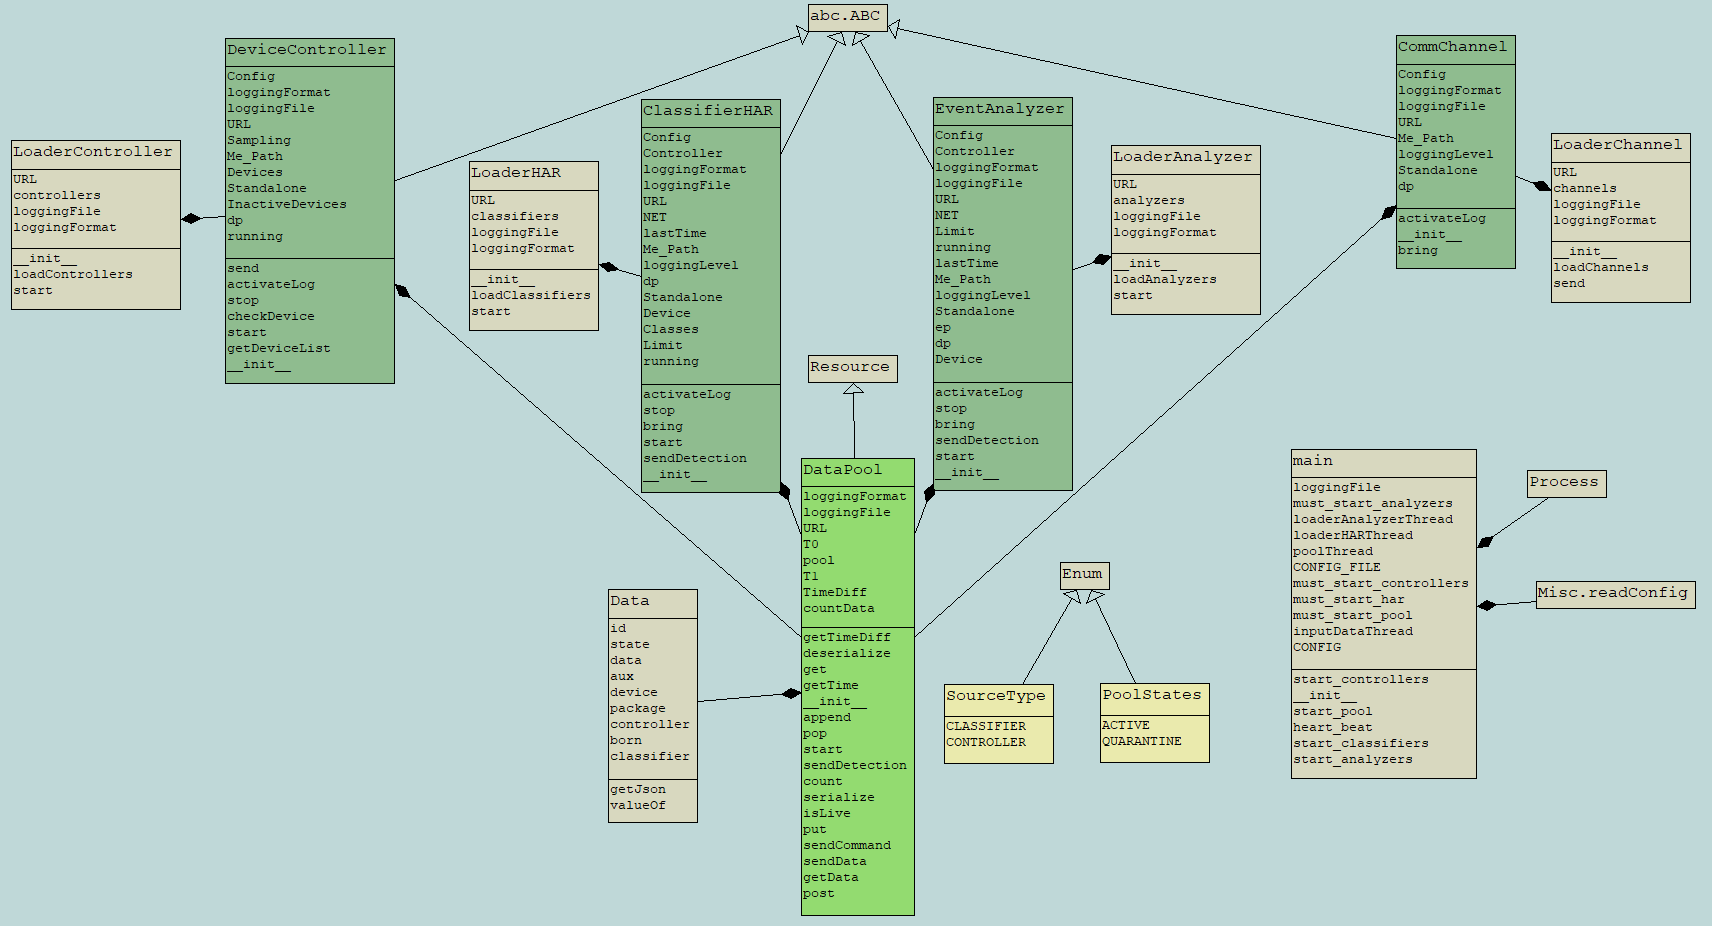
\includegraphics[width=0.9\linewidth]{imgs/03-Architecture/03-FullClassModel.PNG}
        	\caption[Modelo de clases del sistema]{Modelo de clases del sistema. Presenta las la relación y dependencias de la s clases del núcleo y del código base.}
    	    \label{fig:FullClassModel}
        \end{figure}%
        
        En el modelo de clases es se evidencia en verde claro la clase 'DataPool' utilizada por todas las clases base (en verde oscuro) para la transmisión y gestión de los datos del sistema. De igual forma en color más claro las clases cargador (Loader) encargadas de mantener los componentes en funcionamiento y la sanidad del sistema.
        
        La clase 'main', al lado derecho funciona como cargador general del sistema y aunque no hereda de otras clases se encarga de instancias mediante el modelo de hilos (procesos independientes) los servicios de carga (loader) en cada máquina que se ejecute. 
        
    \subsection{Modelo de despliegue}
    \label{sub:DeployModel}
        Visto la ubicación de los artefactos del sistema y mencionado la alta capacidad del sistema para funcionar de forma desacoplada y distribuida la figura \ref{fig:PhysicModel} presenta la forma en que cada componente puede ser dispuesto en diferentes ordenadores sin que se pierda la integridad del sistema.
    
        \begin{figure}[ht!]
        	\centering
        	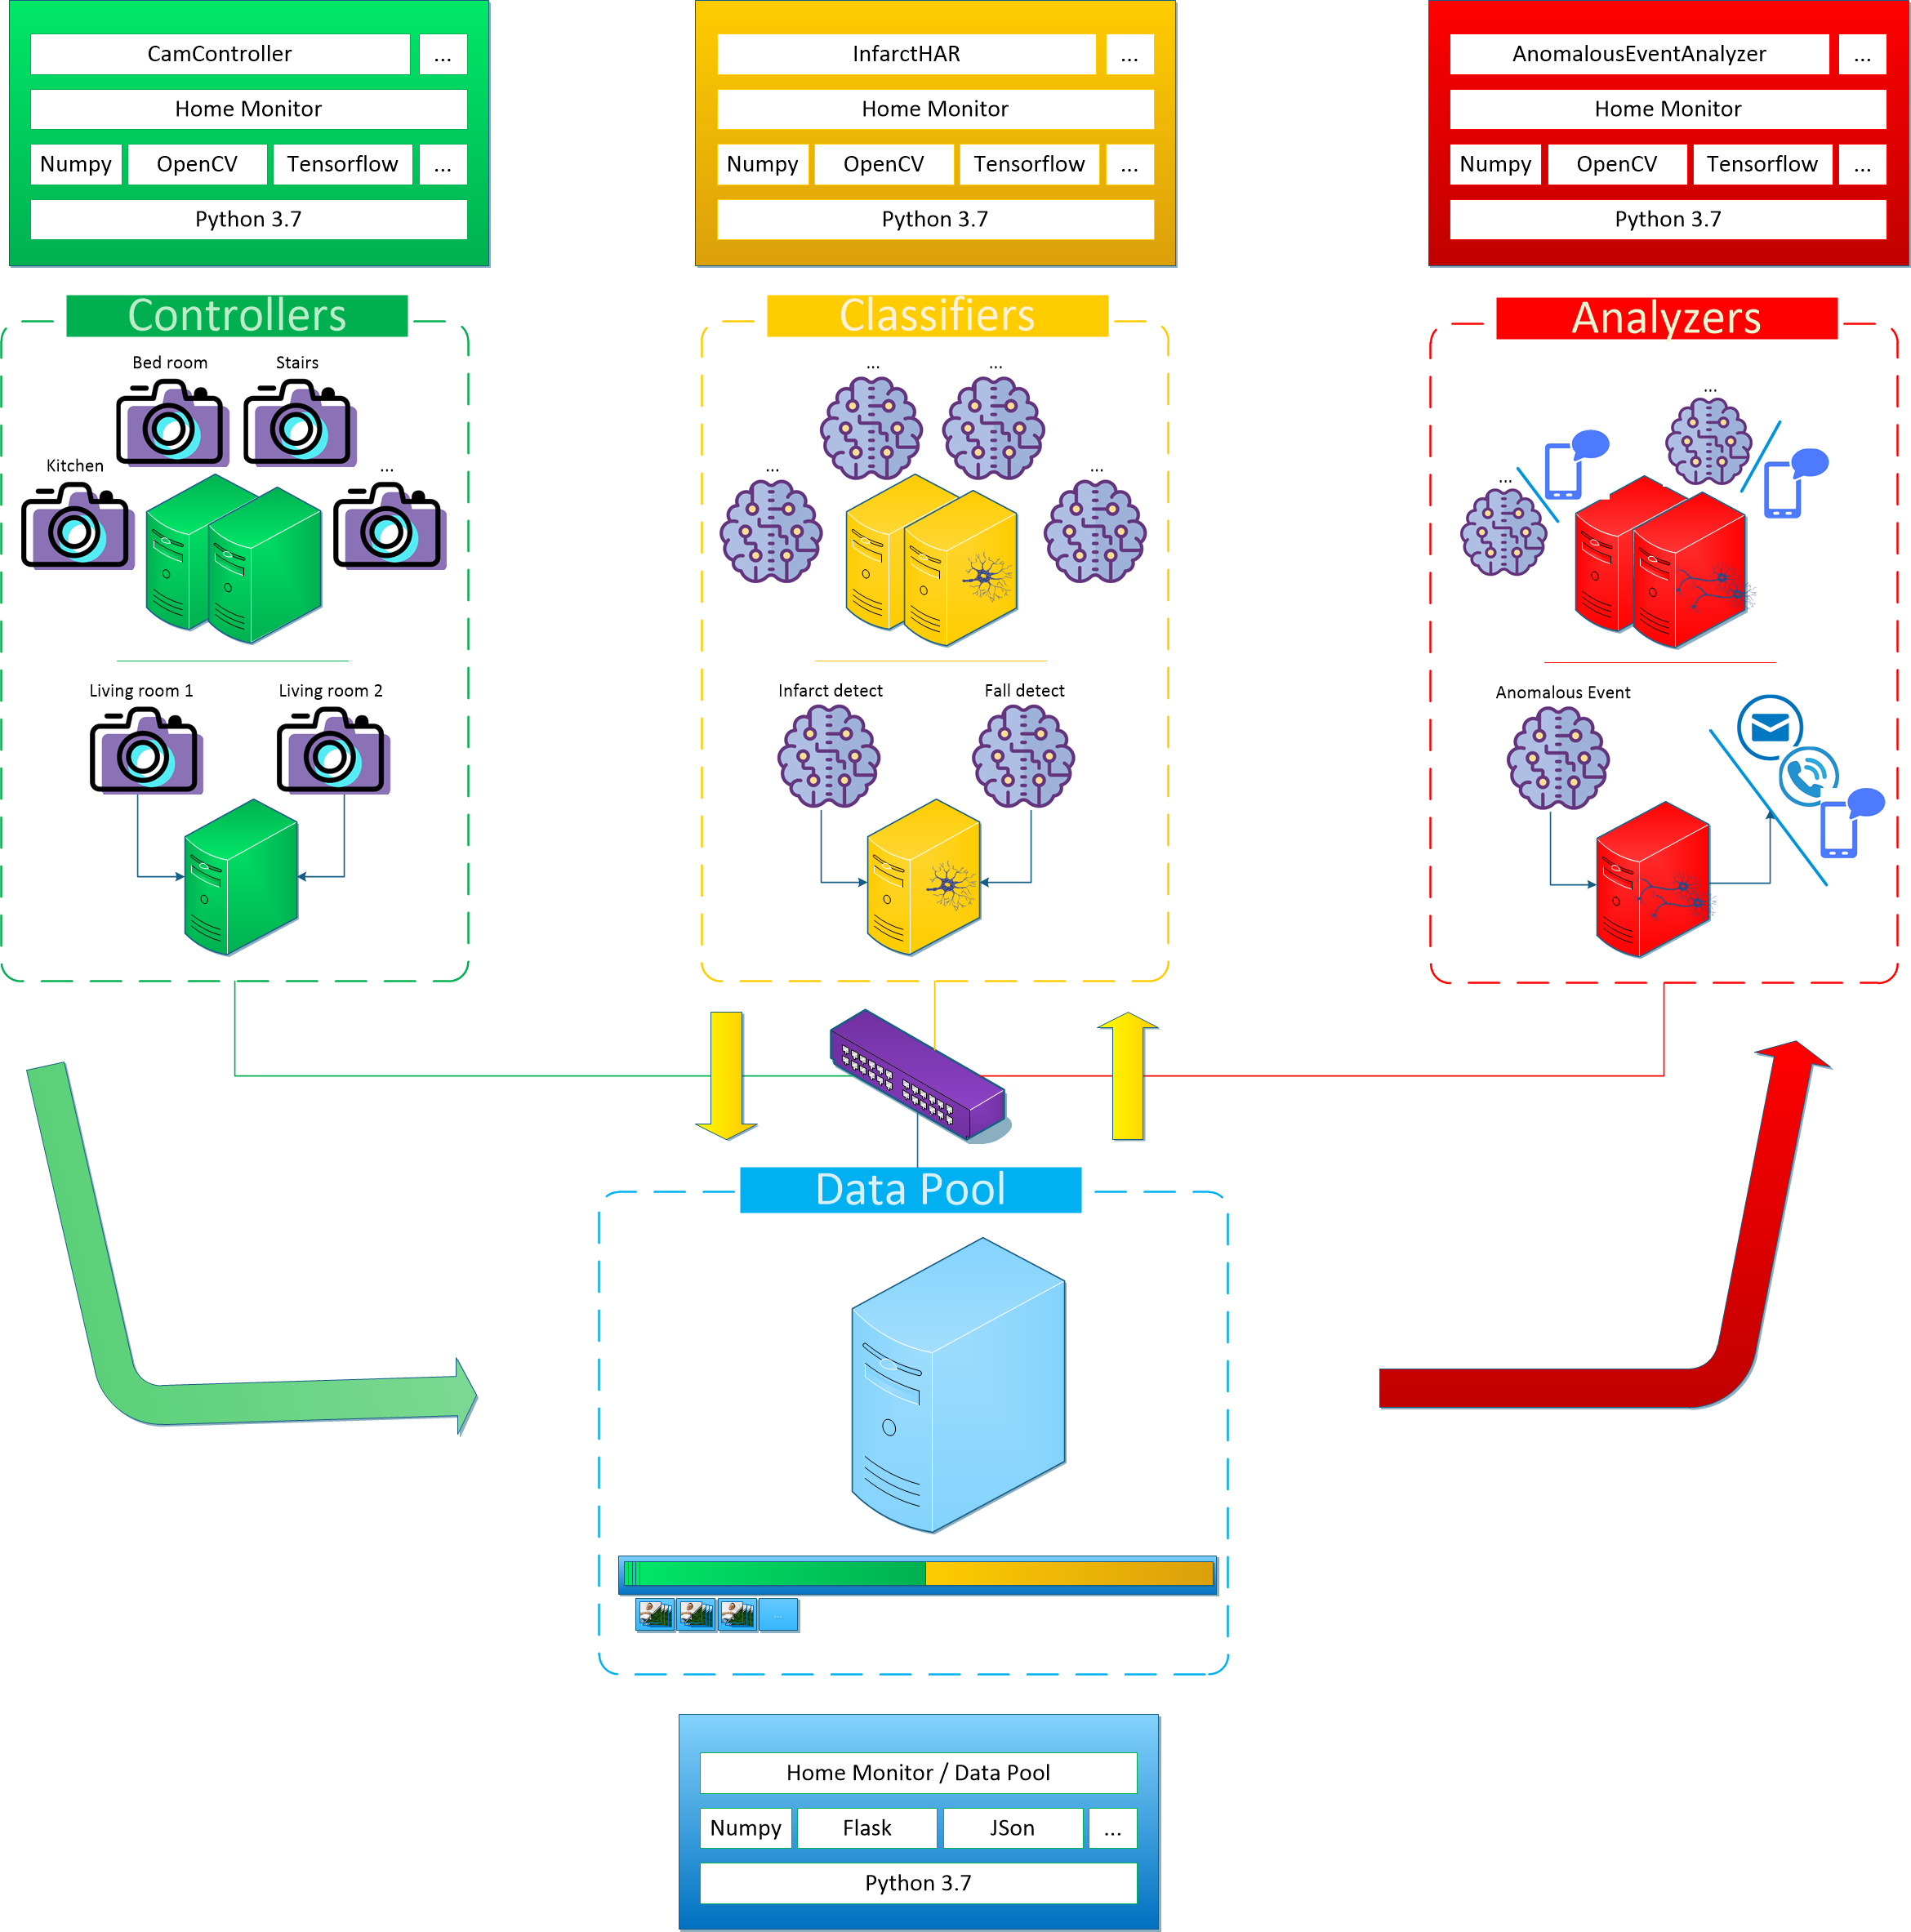
\includegraphics[width=0.9\linewidth]{imgs/03-Architecture/03-PhysicModel.png}
        	\caption[Modelo de despliegue del sistema]{Modelo de despliegue del sistema. Presenta las secciones en que se divide el sistema y los componentes que conforman cada sección. También presenta, de arriba hacia abajo, relación que hay entre cada componente y el sistema general para el intercambio de datos. \textcolor{red}{Cambiar texto recognizers}}
    	    \label{fig:PhysicModel}
        \end{figure}%
    
    Como se muestra en la figura \ref{fig:PhysicModel} cada componente puede ser ejecuto en una máquina independiente, esto significa que es posible usar uno o varios ordenadores para la captura de imágenes, otros para la el procesamiento de los datos capturados. además es posible ejecutar uno o varios analizadores en diferentes máquinas y cada uno con sus canales de notificación independientes.
    
    \newpage

\section{Modelo para la construcción de un componente controlador de dispositivos}
\label{Sec:DeviceControllerTemplate}
    Para asegurar una forma de construcción estándar de nuevos componentes controladores de dispositivos, en este trabajo se definió y desarrollo una plantilla que permite la implementación rápida de un nuevo componente controlador de dispositivos.

    \subsection{Plantilla Controlador de dispositivos}
    \label{sub:TplController}
        
        La plantilla aquí expuesta contiene todos los artefactos necesarios para la creación de nuevos componentes. Cada componente controlador de dispositivos está formado por un directorio que contiene tres archivos como se muestra en la figura \ref{fig:TplControllerFiles}.
    
        \begin{figure}[ht!]
        	\centering
        	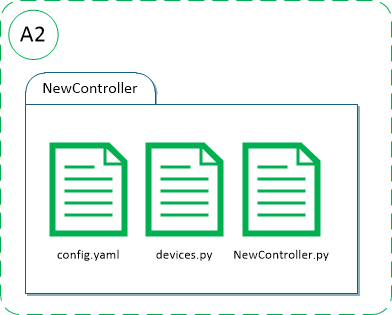
\includegraphics[width=0.5\linewidth]{imgs/03-Architecture/03-TplControllerFiles.png}
        	\caption[Archivos de un componente controlador]{Archivos de un componente controlador.}
    	    \label{fig:TplControllerFiles}
        \end{figure}%
        
        \subsubsection{Archivo de configuración controlador - config.yaml}
        \label{sub2:ConfigFileController}
            Este archivo contiene las variables de configuración y descripción del componente. El sistema usa este archivo para identificar los controladores disponibles y las particularidades de cada uno. La tabla \ref{Tab:ConfigFileController} presenta el listado de atributos disponibles. Es importante mencionar que además de estas cada componente podría adicionar las que le sean necesarias y, de forma autónoma, todas las variables serán cargadas y accesibles una vez el sistema instancie el componente.

            \begin{table}[ht!]
            \caption[Archivo de configuración controlador]{Atributos del archivo de configuración controlador.}
            \label{Tab:ConfigFileController}
            \centering
            \begin{tabular}{ | l l p{6cm} | } 
                \hline
                \textbf{Atributo}       & \textbf{Valor} & \textbf{Descripción} \\ 
                \hline\hline
                \textbf{NAME}           & NewController & Nombre del componente.\\
                \hline
                \textbf{TYPE}           & CONTROLLER    & Tipo de componentye.\\
                \hline
                \textbf{FILE\_CLASS}    & NewController & Nombre del archivo ``py'' donde se encuentra la clase inicial.\\
                \hline
                \textbf{CLASS\_NAME}    & NewController & Clase para cargar el componente (debe heredar de la clase 'DeviceController').\\
                \hline
                \textbf{VERSION}        & 1.0.0         &  Versión del componente.\\
                \hline
                \textbf{ENABLED}        & Y             & Indica si el componente debe o no ser cargado.\\
                \hline
                \textbf{DESCRIPTION}    & ...           & Descripción del componente.\\
                \hline
                \textbf{SAMPLING}       & 0.0           & Tasa de muestreo (en segundos) para la captura de datos del dispositivo.\\
                \hline
                \textbf{CHECK\_TIME}     & 30           &  Tasa de verificación (en segundos) de disponibilidad de dispositivos.\\
                \hline
            \end{tabular}
            \end{table}
            
        \subsubsection{Archivo de dispositivos - devices.yaml}
        \label{sub2:devicesFileController}
            Este archivo contiene la descripción de los dispositivos que serán cargados y de los cuales se obtendrán los datos que procesará el sistema. 

            \lstinputlisting[language=Python, caption={Estructura del archivo de configuración de dispositivos.}, label=Alg:devices]{code/03-Architecture/03-devices.yaml}

            El fragmento de código alg. \ref{Alg:devices} presenta la estructura del archivo. Como se ve muestra cada dispositivo cuenta con tres atributos: \textbf{id} que corresponde al identificador interno del dispositivo, \textbf{name} donde de almacena el nombre con el cual se reconocerá el dispositivo, este nombre podrá ser usado para filtrar las consultas que se hagan a la pila de datos. Finalmente, el atributo \textbf{enabled} indica si el dispositivo debe ser cargado o no. De manera similar, a cada dispositivo se puede asociar las variables que sean necesarias por el componente encargado de su gestión.

        \subsubsection{Clase inicial del controlador - Controller.py}
        \label{sub2:classFileController}
            Esta clase hereda de la clase padre 'DeviceController.py'. Su nombre está compuesto por el nombre del componente seguido de la palabra 'Controller' (sin espacios).
            
            Como se mencionó anteriormente, es en esta clase donde se realiza la captura de datos de los distintos dispositivos y posterior envío a la pila de datos. la plantilla aquí expuesta contiene una copia funcional de este archivo, con todos los métodos que deben ser implementados y los comentarios que sirven de guía al desarrollador de un nuevo componente de este tipo (ver alg. \ref{Alg:NewController}). Adicionalmente, contiene un fragmento de código que permite que el componente sea ejecutado de forma independiente al sistema.
            
            \lstinputlisting[language=Python, caption={Plantilla para un nuevo controlador de dispositivos.}, label=Alg:NewController]{code/03-Architecture/NewController.py}

    \subsection{Implementación de un nuevo controlador de dispositivos}
    \label{sub:DevelopingController}
        
        A continuación, se presentan los pasos el desarrollo de un nuevo componente controlador de dispositivos, partiendo de la plantilla provista.
    
        \begin{itemize}
            \item \textbf{Paso 1}: Creación del componente. Para realizar este paso, basta con ejecutar la siguiente instrucción en la carpeta raíz:
            \begin{itemize}
                \item hm -g controller \textit{$<Name>$}
                \item Ejemplo: hm -g controller \textit{$cam$}
            \end{itemize}
            Esto creará una carpeta con el mismo nombre puesto al nuevo componte más la palabra 'Controller', esta nueva carpeta estará ubicada en la carpeta 'Controllers' como se muestra en la figura \ref{fig:NewController}.
    
            \begin{figure}[ht!]
            	\centering
            	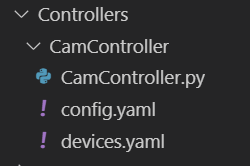
\includegraphics[width=0.4\linewidth]{imgs/03-Architecture/03-NewController.png}
            	\caption[Archivos de un nuevo controlador]{Archivos de un nuevo controlador.}
        	    \label{fig:NewController}
            \end{figure}%
            
            \item \textbf{Paso 2}: Edición de configuraciones. Aunque los archivos de la plantilla están diseñados para que puedan ser funcionales desde el primer momento, será necesario cambiar los valores que se considere necesario para el nuevo componente (ver sección \ref{sub2:ConfigFileController}).
            
            \item \textbf{Paso 3}: El tercer paso consiste en la modificación del archivo \textbf{devices.yaml}, incluyendo los dispositivos que se dispongan en el ordenador donde será ejecutado el componente.
            
            \item \textbf{Paso 4}: Para el último paso, se debe modificar el método '\textbf{getData}', incluyendo la lógica que permita obtener los datos de los dispositivos. El fragmento de código alg. \ref{Alg:NewControler-getData}, presenta un ejemplo de la implementación de este método.

            \lstinputlisting[language=Python, caption={Implementación del método 'getData' en un nuevo controlador.}, label=Alg:NewControler-getData]{code/03-Architecture/03-NewControler-getData.py}
            
            La variable 'self.Devices' contiene el listado de dispositivos cargados. Es importante mencionar que este trabajo facilita la implementación de nuevos componentes realizando tareas de índole general a todos los componente, como son la carga de dispositivos, la serialización de los datos capturados y el envío de los datos. Por tal razón dichas funcionalidades no se encuentran dentro de los artefactos generados en el nuevo componente.
            
            \item \textbf{Paso opcional}: Aunque es opcional, también es recomendable implementar los métodos '\textbf{showData}' y '\textbf{simulateData}' para poder ver los datos capturados cuando el componente se ejecuta en forma independiente al sistema. Para la ejecución de independiente basta con lanzar el archivo de ejecución del componente ($<Name>$\_controller.py) directamente, pues éste ya contiene las instrucciones para ello.
            
        \end{itemize}
        
    \newpage

\section{Modelo para la construcción de un componente de Reconocedor de actividades}
\label{Sec:ClassifierHARTemplate}
    Para asegurar una forma de construcción estándar de nuevos componentes reconocedores de actividades, en este trabajo se definió y desarrollo una plantilla que permite la implementación rápida de este tipo de componentes.

    \subsection{Plantilla Reconocedor de actividades}
    \label{sub:TplHAR}
        
        La plantilla aquí expuesta contiene todos los artefactos necesarios para la creación de nuevos componentes. Cada componente Reconocedor de actividades está formado por un directorio que contiene cinco archivos como se muestra en la figura \ref{fig:TplHARFiles}.
    
        \begin{figure}[ht!]
        	\centering
        	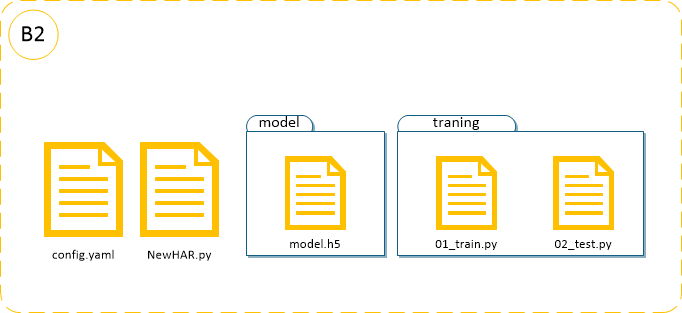
\includegraphics[width=0.8\linewidth]{imgs/03-Architecture/03-TplHARFiles.png}
        	\caption[Archivos de un reconocedor de actividades]{Archivos de un reconocedor de actividades.}
    	    \label{fig:TplHARFiles}
        \end{figure}%
        
        \subsubsection{Archivo de configuración clasificador - config.yaml}
        \label{sub2:ConfigFileHAR}
            Este archivo contiene las variables de configuración y descripción del componente. El sistema usa este archivo para identificar los reconocedores disponibles y sus particularidades. La tabla \ref{Tab:ConfigFileHAR} presenta el listado de atributos disponibles.

            \begin{table}[ht!]
            \caption[Archivo de configuración clasificador]{Atributos del archivo de configuración clasificador.}
            \label{Tab:ConfigFileHAR}
            \centering
            \begin{tabular}{ | l l p{7cm} | } 
                \hline
                \textbf{Atributo}       & \textbf{Valor} & \textbf{Descripción} \\ 
                \hline\hline
                \textbf{NAME}           & NewRecognizer & Nombre del componente.\\
                \hline
                \textbf{TYPE}           & RECOGNIZER    & Tipo componente.\\
                \hline
                \textbf{FILE\_CLASS}    & NewRecognizer & Nombre del archivo 'py', donde está la clase inicial.\\
                \hline
                \textbf{CLASS\_NAME}    & NewRecognizer & Clase para cargar el componente (debe heredar de la clase 'ActivityRecognizer').\\
                \hline
                \textbf{VERSION}        & 1.0.0         &  Versión del componente.\\
                \hline
                \textbf{ENABLED}        & Y             & Indica si el componente debe o no ser cargado.\\
                \hline
                \textbf{DESCRIPTION}    & ...           &  Descripción del componente.\\
                \hline
                \textbf{CLASSES}*       & ...           & Nombre de los eventos detectados.\\
                \hline
                \textbf{MODEL}          & model/model.h5 & Ruta al archivo del entrenamiento.\\
                \hline
                \textbf{FILTER\_NAME}** & ...           & Nombre de un controlador.\\
                \hline
                \textbf{FILTER\_ITEM}** & ...           & Nombre de un dispositivo.\\
                \hline
                \textbf{FILTER\_LIMIT}**& -1            & Cantidad de elementos a consultar cada vez en la pila de datos.\\
                \hline
            \end{tabular}
            \newline
            * Permite personalizar el nombre de los eventos que serán detectados por este componente.\\
            ** Estas variables son opcionales, pero permiten asignar un filtro predeterminado para las consultas que haga este componente a la pila de datos.
            \end{table}
            
        \subsubsection{Clase inicial del clasificador - Recognizer.py}
        \label{sub2:classFileHAR}
            Esta clase hereda de la clase padre 'ActivityRecognizer' y debe implementar los métodos que permitirán la identificación de eventos simples. La plantilla aquí expuesta contiene una copia funcional de este archivo, con todos los métodos que deben ser implementados y los comentarios que sirven de guía al desarrollador de un nuevo componente de este tipo (ver alg. \ref{Alg:NewRecognizer}). Adicionalmente, contiene un fragmento de código que permite que el componente sea ejecutado de forma independiente al sistema.
            
            \lstinputlisting[language=Python, caption={Plantilla para un nuevo Reconocedor de actividades.}, label=Alg:NewRecognizer]{code/03-Architecture/NewRecognizer.py}

        \subsubsection{Entrenamientos de inteligencia artificial - models}
        \label{sub2:modelFileHAR}
            Aunque en la plantilla no se provee un archivo con un entrenamiento, si cuenta con una sub carpeta donde podrán alojarse los archivos relacionados con entrenamientos previos para su futura distribución.
        
        \subsubsection{Plantillas para entrenamiento y prueba}
        \label{sub2:trainFileHAR}
            Aunque los tres primeros archivos ('config.yaml', \_Recognizer y model), son suficientes para el correcto funcionamiento de un componente de reconocimiento de actividad humana, en este trabajo se incluyó, dentro de los archivos de la plantilla dos más: '01\_train.py' (archivo de entrenamiento) y '02\_test.py' (archivo de prueba). Estos archivos contemplan el proceso de entrenamiento y prueba de una nueva red neuronal para lo cual bastaría con contar el conjunto de datos de entrenamiento (ver \ref{Sec:TrainValTestDataset}).
            
            En primera instancia el archivo '01\_train.py' contiene una red neuronal, previamente diseñada para la detección de eventos u objetos en imágenes. En este archivo se definen tres variables:
            \begin{itemize}
                \item \textbf{INPUT\_PATH\_TRAIN}: En esta variable se indicará la ruta donde se encuentran las imágenes de entrenamiento. Las imágenes deberán estar agrupadas en sub carpetas, donde se asumirá cada sub carpeta como una clase o categoría.
                \item \textbf{INPUT\_PATH\_VAL}: Variable similar a la anterior, pero debe contener un conjunto diferente de imágenes, con las cuales se irá validando la precisión del aprendizaje durante el entrenamiento mismo.
                \item \textbf{OUTPUT\_DIR}: Ruta a la carpeta donde el modelo o archivo de aprendizaje será almacenado durante proceso de entrenamiento.
            \end{itemize}
            
            Además de las variables mencionadas, el archivo de entrenamiento, contiene algunas más que permiten, entre otras cosas: definir la cantidad de épocas de entrenamiento, el numero de clases a detectar o la tasa de aprendizaje.
            
            El segundo archivo, '02\_test.py' contiene la lógica para definir que tan bueno es el aprendizaje obtenido en el entrenamiento, con un conjunto de imágenes no usado anteriormente, durante el entrenamiento o validación.
            
            Para la generalización del uso de este archivo se tienen tres variables principales: 
            
            \begin{itemize}
                \item \textbf{INPUT\_PATH\_TEST}: Ruta a la carpeta con las imágenes de prueba, agrupadas bajo el mismo criterio que las imágenes de entrenamiento.
                \item \textbf{MODEL\_PATH}: Ruta al archivo modelo, generado durante el entrenamiento.
                \item \textbf{CLASSES}: Listado de clases a identificar.
            \end{itemize}
            
    \subsection{Implementación de un nuevo Reconocedor de actividades}
    \label{sub:DevelopingHAR}
        A continuación, se presentan los pasos el desarrollo de un nuevo componente Reconocedor de actividades, partiendo de la plantilla provista en este trabajo.
    
        \begin{itemize}
            \item \textbf{Paso 1}: Creación del componente. Para realizar este paso, basta con ejecutar la siguiente instrucción en la carpeta raíz:
            \begin{itemize}
                \item hm -g recognizer \textit{$<Name>$}
                \item Ejemplo: hm -g recognizer \textit{$rgbInfarct$}
            \end{itemize}
            Esto creará una carpeta con el mismo nombre puesto al nuevo componte más la palabra 'Recognizer', esta nueva carpeta estará ubicada en la carpeta 'Recognizers' como se muestra en la figura \ref{fig:NewHAR}.
    
            \begin{figure}[ht!]
            	\centering
            	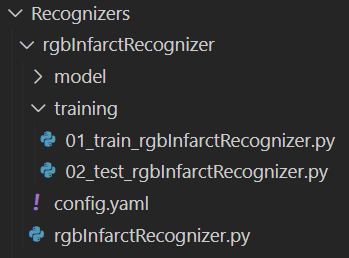
\includegraphics[width=0.4\linewidth]{imgs/03-Architecture/03-NewHAR.png}
            	\caption[Archivos de un nuevo clasificador HAR]{Archivos de un nuevo clasificador HAR.}
        	    \label{fig:NewHAR}
            \end{figure}%
            
            \item \textbf{Paso 2}: Edición de configuraciones. Aunque los archivos de la plantilla están diseñados para que puedan ser funcionales desde el primer momento, será necesario cambiar los valores que se considere necesario para el nuevo componente (ver sección \ref{sub2:ConfigFileHAR}).
            
            \item \textbf{Paso 3}: Entrenamiento. En este paso será necesario seguir los lineamientos para la creación de un conjunto de datos de entrenamiento (ver sección \ref{Sec:TrainValTestDataset}).
            
            Una vez se disponga de los datos de entrenamiento, dependiendo el tipo de datos, podrá hacerse uso del archivo '01\_train.py' para la generación del aprendizaje. 
            
            En caso de disponer de un entrenamiento previo, bastará con poner el archvio de entrenamiento en la carpeta 'model'.
            
            \item \textbf{Paso 4}: Una vez generado el archivo de entrenamiento, se debe modificar el método '\textbf{predict}', incluyendo la lógica que permita identificar eventos y retornar las clases correspondientes. El fragmento de código alg. \ref{Alg:NewHAR-predict}, presenta un ejemplo de la implementación de este método.

            \lstinputlisting[language=Python, caption={Implementación del método 'predict' en un nuevo clasificador.}, label=Alg:NewHAR-predict]{code/03-Architecture/03-NewHAR-predict.py}
            
            La variable 'self.MODEL' contiene la red neuronal con el entrenamiento previo. La variable 'self.CLASSES' contiene la lista de clases que es posible detectar por el modelo, esta lista deberá estar definida en el archivo 'config.yaml' del propio componente. Es importante mencionar que este trabajo facilita la implementación de nuevos componentes realizando tareas de índole general a todos los componente, como son la carga del entrenamiento de la red y el envío de los eventos detectados a la pila de datos. Por tal razón dichas funcionalidades no se encuentran dentro de los artefactos generados en el nuevo componente.
            
            \item \textbf{Paso opcional}: Aunque es opcional, también es recomendable implementar los métodos '\textbf{showData}' y '\textbf{simulateData}' para poder verificar la correcta inferencia de eventos, cuando el componente se ejecuta en forma independiente al sistema. Para la ejecución de independiente basta con lanzar el archivo de ejecución del componente (\_Recognizer.py), pues éste ya contiene las instrucciones para ello.
            
        \end{itemize}
        
    \newpage
    
\section{Modelo para la construcción de un componente analizador de eventos}
\label{Sec:EventAnalyzerTemplate}
    En esta sección del documento, se presentará la plantilla que permite la implementación rápida de un nuevo componente para el análisis de eventos.

    \subsection{Plantilla analizador}
    \label{sub:TplAnalyzer}
        
        La plantilla aquí expuesta contiene todos los artefactos necesarios para la creación de nuevos componentes. Cada componente analizador de eventos está formado por un directorio que contiene tres archivos como se muestra en la figura \ref{fig:TplAnalyzerFiles}.
    
        \begin{figure}[ht!]
        	\centering
        	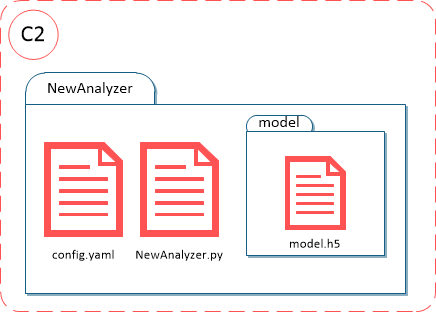
\includegraphics[width=0.7\linewidth]{imgs/03-Architecture/03-TplAnalyzerFiles.png}
        	\caption[Archivos de un analizador de eventos]{Archivos de un analizador de eventos.}
    	    \label{fig:TplAnalyzerFiles}
        \end{figure}%
        
        \subsubsection{Archivo de configuración analizador - config.yaml}
        \label{sub2:ConfigFileAnalyzer}
            Este archivo contiene las variables de configuración y descripción del componente. El sistema usa este archivo para identificar los analizadores disponibles y sus particularidades. La tabla \ref{Tab:ConfigFileAnalyzer} presenta el listado de atributos disponibles.

            \begin{table}[ht!]
            \caption[Archivo de configuración analizador]{Atributos del archivo de configuración analizador.}
            \label{Tab:ConfigFileAnalyzer}
            \centering
            \begin{tabular}{ | l l p{7cm} | } 
                \hline
                \textbf{Atributo}       & \textbf{Valor} & \textbf{Descripción} \\ 
                \hline\hline
                \textbf{NAME}           & NewAnalyzer & Nombre del componente.\\
                \hline
                \textbf{TYPE}           & ANALYZER    & Tipo componente.\\
                \hline
                \textbf{FILE\_CLASS}    & NewAnalyzer & Nombre del archivo 'py', donde está la clase inicial.\\
                \hline
                \textbf{CLASS\_NAME}    & NewAnalyzer & Clase para cargar el componente (debe heredar de la clase 'EventAnalyzer').\\
                \hline
                \textbf{VERSION}        & 1.0.0         &  Versión del componente.\\
                \hline
                \textbf{ENABLED}        & Y             & Indica si el componente debe o no ser cargado.\\
                \hline
                \textbf{DESCRIPTION}    & ...           &  Descripción del componente.\\
                \hline
                \textbf{MODEL}          & model/model.h5 & Ruta al archivo del entrenamiento.\\
                \hline
                \textbf{FILTER\_NAME}** & ...           & Nombre de un reconocedor.\\
                \hline
                \textbf{FILTER\_ITEM}** & ...           & Sub Nombre de un reconocedor.\\
                \hline
                \textbf{FILTER\_LIMIT}**& -1            & Cantidad de elementos a consultar cada vez en la pila de datos.\\
                \hline
            \end{tabular}
            \newline
            ** Estas variables son opcionales, pero permiten asignar un filtro predeterminado para las consultas que haga este componente a la pila de datos.
            \end{table}

        \subsubsection{Clase inicial del Analizador - \_Analyzer.py}
        \label{sub2:classFileAnalyzer}
            Esta clase hereda de la clase padre 'EventAnalyzer.py'. Su nombre está compuesto por el nombre del componente seguido de la palabra 'Analyzer' (sin espacios).
            
            En esta clase se deben implementar los métodos para analizar los eventos simples detectados por los clasificadores e identificar situaciones anómalas. la plantilla aquí expuesta contiene una copia funcional de este archivo, con todos los métodos que deben ser implementados y los comentarios que sirven de guía al desarrollador de un nuevo componente de este tipo (ver alg. \ref{Alg:NewAnalyzer}). Adicionalmente, contiene un fragmento de código que permite que el componente sea ejecutado de forma independiente al sistema.
            
            \lstinputlisting[language=Python, caption={Plantilla para un nuevo Analizador de Eventos.}, label=Alg:NewAnalyzer]{code/03-Architecture/NewAnalyzer.py}

        \subsubsection{Entrenamientos de inteligencia artificial - models}
        \label{sub2:modelFileAnalyzer}
            Aunque en la plantilla no se provee un archivo con un entrenamiento, la plantilla si cuenta con una sub carpeta donde podrán alojarse dichos archivos luego del entrenamiento de forma que puedan ser parte integra del modulo para su futura distribución.
        
    \subsection{Implementación de un nuevo analizador de eventos}
    \label{sub:DevelopingAnalyzer}
        
        A continuación, se presentan los pasos el desarrollo de un nuevo componente analizador de eventos, partiendo de la plantilla provista en este trabajo.
    
        \begin{itemize}
            \item \textbf{Paso 1}: Creación del componente. Para realizar este paso, basta con ejecutar la siguiente instrucción en la carpeta raíz:
            \begin{itemize}
                \item hm -g analyzer Name
            \end{itemize}
            Esto creará una carpeta con el mismo nombre puesto al nuevo componte más la palabra 'Analyzer', esta nueva carpeta estará ubicada en la carpeta 'Analyzers' como se muestra en la figura \ref{fig:NewAnalyzer}.
    
            \begin{figure}[ht!]
            	\centering
            	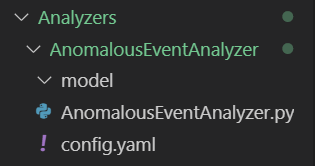
\includegraphics[width=0.4\linewidth]{imgs/03-Architecture/03-NewAnalyzer.png}
            	\caption[Archivos de un nuevo analizado de eventos]{Archivos de un nuevo analizador de eventos.}
        	    \label{fig:NewAnalyzer}
            \end{figure}%
            
            \item \textbf{Paso 2}: Edición de configuraciones. Aunque los archivos de la plantilla están diseñados para que puedan ser funcionales desde el primer momento, será necesario cambiar los valores que se considere necesario para el nuevo componente (ver sección \ref{sub2:ConfigFileAnalyzer}).
            
            \item \textbf{Paso 3}: Entrenamiento. Este paso depende enteramente del alcance deseado para el componente, sin embargo, se asume que el resultado es un archivo de entrenamiento. Este entrenamiento debe ser almacenado en la sub carpeta 'model'.
            
            \item \textbf{Paso 4}: Una vez generado el archivo de entrenamiento, se debe modificar el método '\textbf{analyze}', incluyendo la lógica que permita identificar situaciones complejas a partir de los eventos simples. El fragmento de código alg. \ref{Alg:NewAnalyzer-analyze}, presenta un ejemplo de la implementación de este método.

            \lstinputlisting[language=Python, caption={Implementación del método 'analyze' en un nuevo analizador.}, label=Alg:NewAnalyzer-analyze]{code/03-Architecture/03-NewAnalyzer-analyze.py}
            
            La variable 'self.MODEL' contiene la red neuronal con el entrenamiento previo. Es importante mencionar que este trabajo facilita la implementación de nuevos componentes realizando tareas de índole general a todos los componente, como son la carga del entrenamiento de la red y el envío de mensajes a los notificadores. Por tal razón dichas funcionalidades no se encuentran dentro de los artefactos generados en el nuevo componente.
            
            \item \textbf{Paso opcional}: Aunque es opcional, también es recomendable implementar los métodos '\textbf{showData}' y '\textbf{simulateData}' para poder verificar el correcto análisis de los eventos, cuando el componente se ejecuta en forma independiente al sistema. Para la ejecución de independiente basta con lanzar el archivo de ejecución del componente (\_Analyzer.py), pues éste ya contiene las instrucciones para ello.
            
        \end{itemize}
        
    \newpage
    
\section{Modelo para la construcción de un componente de notificación}
\label{Sec:NotifierChannelTemplate}

    En esta sección del documento, se presentará tanto la plantilla que permite la implementación rápida de un nuevo componente para el envío de los mensajes relacionados con las inferencias hechas por el analizador de eventos, como su implementación.

    \subsection{Plantilla notificador}
    \label{sub:TplChannel}
        
        La plantilla aquí expuesta contiene todos los artefactos necesarios para la creación de nuevos componentes. Cada componente notificador está formado por un directorio que contiene dos archivos como se muestra en la figura \ref{fig:TplChannelFiles}.
    
        \begin{figure}[ht!]
        	\centering
        	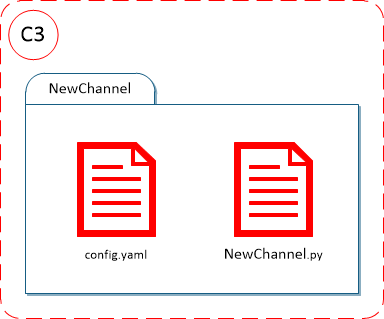
\includegraphics[width=0.6\linewidth]{imgs/03-Architecture/03-TplChannelFiles.png}
        	\caption[Archivos de un notificador]{Archivos de un notificador.}
    	    \label{fig:TplChannelFiles}
        \end{figure}%
        
        \subsubsection{Archivo de configuración notificador - config.yaml}
        \label{sub2:ConfigFileChannel}
            Este archivo contiene las variables de configuración y descripción del componente. El sistema usa este archivo para identificar los notificadores disponibles y sus particularidades. La tabla \ref{Tab:ConfigFileChannel} presenta el listado de atributos disponibles.

            \begin{table}[ht!]
            \caption[Archivo de configuración del componente notificador]{Atributos del archivo de configuración del componente notificador.}
            \label{Tab:ConfigFileChannel}
            \centering
            \begin{tabular}{ | l l p{7cm} | } 
                \hline
                \textbf{Atributo}       & \textbf{Valor} & \textbf{Descripción} \\ 
                \hline\hline
                \textbf{NAME}           & NewChannel & Nombre del componente.\\
                \hline
                \textbf{TYPE}           & ANALYZER    & Tipo componente.\\
                \hline
                \textbf{FILE\_CLASS}    & NewChannel & Nombre del archivo 'py', donde está la clase inicial.\\
                \hline
                \textbf{CLASS\_NAME}    & NewChannel & Clase para cargar el componente (debe heredar de la clase 'CommChannel').\\
                \hline
                \textbf{VERSION}        & 1.0.0         &  Versión del componente.\\
                \hline
                \textbf{ENABLED}        & Y             & Indica si el componente debe o no ser cargado.\\
                \hline
                \textbf{DESCRIPTION}    & ...           &  Descripción del componente.\\
                \hline
                \textbf{FROM}*      & ...  & Usuario o cuenta de origen .\\
                \hline
                \textbf{PASSWORD}*  & ...  & Clave del usuario que envía el mensaje.\\
                \hline
                \textbf{TO}*        & ...  & Destinatarios principales.\\
                \hline
                \textbf{CC}*        & ...  & Destinatarios copiados.\\
                \hline
                \textbf{BCC}*       & ...  & Destinatarios ocultos.\\
                \hline
                \textbf{SUBJECT}*   & ...  & Plantilla de asunto, puede usar tokens o palabras clave para remplazar variables con valores entregados por el analizador.\\
                \hline
                \textbf{MESSAGE}*   & ...  & Plantilla de mensaje, puede usar tokens o palabras clave para remplazar variables con valores entregados por el analizador.\\
                \hline
            \end{tabular}
            \newline
            * Estas variables son opcionales y podrían variar según las necesidades del componente.
            \end{table}

        \subsubsection{Clase inicial del clasificador - \_Channel.py}
        \label{sub2:classFileChannel}
            Esta clase hereda de 'CommChannel.py'. Su nombre está compuesto por el nombre del componente seguido de la palabra 'Channel' (sin espacios).
            
            En esta clase se deben implementar los métodos necesarios para el envío de un mensaje por un canal concreto, por ejemplo correo electrónico o SMS. la plantilla aquí expuesta contiene una copia funcional de este archivo, con todos los métodos que deben ser implementados y los comentarios que sirven de guía al desarrollador de un nuevo componente de este tipo (ver alg. \ref{Alg:NewAnalyzer}). Adicionalmente, contiene un fragmento de código que permite que el componente sea ejecutado de forma independiente al sistema.
            
            \lstinputlisting[language=Python, caption={Plantilla para un nuevo Canal de notificaciones.}, label=Alg:NewChannel]{code/03-Architecture/NewChannel.py}
            
    \subsection{Implementación de un nuevo notificador}
    \label{sub:DevelopingChannel}
        
        A continuación, se presentan los pasos el desarrollo de un nuevo componente notificador, partiendo de la plantilla provista en este trabajo.
    
        \begin{itemize}
            \item \textbf{Paso 1}: Creación del componente. Para realizar este paso, basta con ejecutar la siguiente instrucción en la carpeta raíz:
            \begin{itemize}
                \item hm -g channel Name
            \end{itemize}
            Esto creará una carpeta con el mismo nombre puesto al nuevo componte más la palabra 'Channel', esta nueva carpeta estará ubicada en la carpeta 'Channels' como se muestra en la figura \ref{fig:NewChannel}.
    
            \begin{figure}[ht!]
            	\centering
            	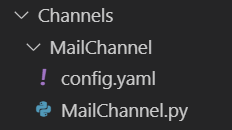
\includegraphics[width=0.4\linewidth]{imgs/03-Architecture/03-NewChannel.png}
            	\caption[Archivos de un nuevo notificador]{Archivos de un nuevo notificador.}
        	    \label{fig:NewChannel}
            \end{figure}%
            
            \item \textbf{Paso 2}: Edición de configuraciones. Aunque los archivos de la plantilla están diseñados para que puedan ser funcionales desde el primer momento, será necesario cambiar los valores que se considere necesario para el nuevo componente (ver sección \ref{sub2:ConfigFileChannel}).
            
            \item \textbf{Paso 3}: El último paso necesario en el desarrollo del componente es la implementación del método '\textbf{trySend}', incluyendo la lógica que permita el envío de mensajes por un canal determinado. El fragmento de código alg. \ref{Alg:NewChannel-send}, presenta un ejemplo de la implementación de este método.

            \lstinputlisting[language=Python, caption={Implementación del método 'send' en un nuevo componente notificador.}, label=Alg:NewChannel-send]{code/03-Architecture/03-NewChannel-send.py}
            
        \end{itemize}
        
    \newpage

\section{Creación de conjuntos de datos para entrenamientos y pruebas}
\label{Sec:TrainValTestDataset}
    Dentro del proceso de creación de sistemas basados en estrategias de inteligencia artificial, uno de los puntos más importantes consiste en contar con un adecuado conjunto de datos tanto para el entrenamiento como para la validación del entrenamiento. 
    
    Debido a lo anterior y, teniendo en cuenta que este trabajo esta pensado para ser escalado, ampliando sus funcionalidades, algunas de ellas involucrando algoritmos de inteligencia artificial, este trabajo contempla la inclusión de conjuntos de datos variados así como la orientación para la creación de nuevos conjuntos, asegurando la aplicación de buenas prácticas.
    
    \subsection{Selección de datos}
    \label{sub:DatasetSelection}
    
    \subsection{División del conjunto de datos: Entrenamiento, Validación y Pruebas}
    \label{sub:DatasetSplit}
    
    \subsection{Aumento de datos}
    \label{sub:DatasetAugmented}
    
    \newpage

\section{Funcionalidades auxiliares}
\label{Sec:Tools}
    Desde su concepción, este proyecto fue pensado como un marco de trabajo que no solo brindará una funcionalidad concreta, sino que también presentará una arquitectura altamente escalable y desacoplable para interconectar los componentes que se integren al sistema, además de un conjunto de herramientas que permitan su extensión. En este capítulo serán presentadas algunas funcionalidades que pueden ser utilizadas tanto en la construcción de nuevos módulos como en el la elaboración de conjuntos de datos de entrenamiento, siguiendo los lineamientos expuestos en secciones anteriores.
    
    Siguiendo con las directrices de arquitectura, en el directorio 'Tools' (ver fig. \ref{fig:SystemDirectories}), de las carpetas del núcleo del sistema, se encuentran las diferentes clases con funcionalidades utilitarias. en este directorio se encuentran: la clase '\textbf{Misc}' que contiene las funciones de índole más general. La clases '\textbf{DataSplit}' y '\textbf{DataAugmented}' que facilitan el proceso de elaboración de conjuntos de datos. Por mencionar algunas, todas serán explicadas a continuación.
    
    \subsection{Utilidades varias - Misc.py}
    \label{sub:MiscClass}
        La clase '\textbf{Misc}' contiene las funcionalidades más diversas del sistema, de forma que al ser importada en los futuros desarrollos se cuente con la mayor cantidad de funcionalidades. Las funcionalidades disponibles son:
    
        \begin{longtable}[c]{ p{7cm} p{7cm} }
            \caption[Métodos de la clase Misc]{Métodos de la clase \textbf{Misc}.} \\ \toprule
            %\textbf{} & \textbf{}\\ \toprule           
            \endfirsthead
            \multicolumn{2}{c}{\textit{\textsl{(Viene de la página anterior)}}} \\
             \\ \toprule
            %\textbf{columna 1} & \textbf{columna 2} \\ \toprule 
            \endhead
            \multicolumn{2}{c}{\textsl{\textit{(Continúa en la página siguiente)}}}\\
            \endfoot
            %\multicolumn{2}{c}{\textit{\textsl{(Texto Footer)}}} \\
            \endlastfoot
            \hline
                    \multicolumn{2}{|c|}{\textbf{Gestión de archivos}}\\ 
                    \hline\hline
                    lsFolders(path=getcwd()) & Retorna una lista con las carpetas que están en una ruta.\\
                    \hline
                    lsFiles(path=getcwd()) & Retorna una lista con los archivos que están en una ruta.\\
                    \hline
                    existsFile(fileName, path=getcwd()) & Retorna verdadero si el archivo existe en la ruta enviada en caso contrario retorna falso. si la ruta no se entrega se revisa la carpeta actual.\\
                    \hline
                    createFolders(path) & Crea una carpeta en la ruta enviada, si las carpetas padre no existen las crea hasta completar toda la ruta.\\
                    \hline
                    saveByType(data, t:str, path:str) & Toma los datos almacenados en el parámetro 'data' y genera un archivo del tipo (t) en la ruta (path) designada. Los tipos posibles son: image, csv. Es útil para el almacenamiento de los datos enviados a la pila de datos.\\
                    
                    \hline\hline\hline
                    \multicolumn{2}{|c|}{\textbf{Gestión de configuraciones}}\\ 
                    \hline\hline
                    readConfig(fileName) & Lee un archivo timo 'yaml' y retorna un objeto con los atributos cargados.\\
                    \hline
                    showConfig(config) & Muestra los valores de un objeto de configuración.\\
                    \hline
                    importModule(path:str, moduleName:str, className:str=None): & Carga durante la ejecución un módulo, de forma que éste no tenga que existir en tiempo d desarrollo o que tenga que estar en memoria en todo momento.\\
                    \hline
                    loggingConf(loggingLevel=logging.INFO, loggingFile=None, loggingFormat=None) & Asigna las configuraciones para el manejo de log del sistema.\\
                    
                    \hline\hline\hline
                    \multicolumn{2}{|c|}{\textbf{Aplicación de patrones}}\\ 
                    \hline\hline
                    singleton(cls) & Asigna el patrón 'singleton'\index{singleton} a una clase, de forma que solo pueda existir una instancia de la misma durante la ejecución del programa.\\
                    
                    \hline\hline\hline
                    \multicolumn{2}{|c|}{\textbf{Varios}}\\ 
                    \hline\hline
                    hasKey(dict, key, default) & Si una variable existe en un diccionario retorna su valor, en caso contrario retorna el valor 'default'.\\
                    \hline
                    toBool(value:str) & Convierte diferentes texto a tipo 'bool', esto es especialmemnte útil en la lectura de variables de configuración puede poner cosas como: 'true', '1', 't', 'y', 'yes', 'yeah', 'yup', 'certainly' o 'uh-huh' .\\
                    \hline
                    randomString(stringLength=10) & Retorna una cadena de texto aleatorio del tamaño indicado, Útil para la generación de ids.\\
                    \hline
       
            \label{Tab:MiscMethods}
        \end{longtable}
        
    \subsection{Segmentación de los datos - DataSplit.py}
    \label{sub:DataSplitClass}
        Esta clase permite la separación de los datos que se van a utilizar para el entrenamiento en tres grupos (Entrenamiento, Validación y Prueba), siguiendo los lineamientos descritos en la sección \ref{sub:DatasetSplit}. Como se mencionó, es recomendable realizar esta tarea antes de un aumento de datos para evitar la mezcla de datos en los subconjuntos.
        
        Para el funcionamiento de esta basta con modificar el valor las siguientes variables:
        \begin{itemize}
            \item \textbf{TYPE}: Indica el tipo de dato a segmentar, Puede tomar el valor de 'images' o 'csv'.
            \item \textbf{INPUT\_PATH}: Ruta donde están los datos originales.
            \item \textbf{OUTPUT\_PATH}: Ruta de destino, aquí se crearan las tres subcarpetas de la segmentación en caso de imágenes o los tres archivos en caso de ser un archivo 'csv'.
            \item \textbf{TRAIN}: Porcentaje del conjunto original asignado al entrenamiento, ejemplo 0.7.
            \item \textbf{VAL}: Porcentaje del conjunto original asignado a la validación, ejemplo 0.15.
            \item \textbf{TEST}: Porcentaje del conjunto original asignado a las pruebas, ejemplo 0.15.
        \end{itemize}
        
    \subsection{Segmentación de los datos - DataAugmented.py}
    \label{sub:DataAugmentedClass}
        Esta clase permite el aumentar la cantidad de ejemplo de una muestra a partir de pequeñas modificaciones de cada uno de lo datos. Actualmente esta clase solo aplica para imágenes,
        
        Para el uso de esta clase es necesario modificar el valor de las siguientes variables:
        \begin{itemize}
            \item \textbf{INPUT\_PATH}: Ruta donde están los datos originales.
            \item \textbf{OUTPUT\_PATH}: Ruta de destino, aquí se almacenarán los archivos modificados.
            \item \textbf{QUANTITY}: Cantidad de datos nuevos a generar.
        \end{itemize}
    
    \newpage

